\documentclass[12pt,oneside]{book}

\usepackage[dvips,letterpaper,margin=0.75in,bottom=0.75in]{geometry}
\usepackage{cite}
\usepackage{slashed}
\usepackage{graphicx}
\usepackage{amsmath}
\usepackage{enumitem}
\usepackage{amsthm}
\theoremstyle{definition}

\usepackage[american,fulldiode]{circuitikz}
\tikzset{component/.style={draw,thick,circle,fill=white,minimum size =0.75cm,inner sep=0pt}}
%\newtheorem{env-name}[other_env]{label-text}
\newtheorem{measurement}{Measurement}[chapter]
\newtheorem{plot}{Plot}[chapter]
\newtheorem{example}{Example}[chapter]
\newtheorem{print}{Print}[chapter]
\newtheorem{calculation}{Calculation}[chapter]


\begin{document}
\ctikzset{bipoles/thickness=1}
\ctikzset{bipoles/length=.6cm}

\title{Physics 80 Lab Manual}
\author{version 13.5}
\maketitle
%\input{intro_python.tex}
\chapter{Arrays and Plotting}

\section{Introduction}

\section{Preparation}

This lab will rely on the material from Sections 1.4.1 to 1.4.2 and
1.5.1 to 1.5.2 of the Scientific Python Lecture notes.  This is the
first lab that relies on inline plotting, so make sure you are
starting your notebook with the ``line magic'':
\begin{python}
  %pylab inline
\end{python}
This will load the numpy library as np, the matplotlib.pyplot library
as plt, and setup the matplotlib backend to imbed plots in your
notebook.

A Numpy array is a grid of values.  Unlike Python lists, the elements
of a numpy array all have the same data type, which makes them much
more computionally efficient.  The numpy library provides a wide range
of analysis tools that are mostly centered on the numpy array type.
Numpy arrays can be constructed from a Python list:
\begin{python}
a = np.array([1.3,7.2,4.1,0.0])
b = np.array([[1,2],[3,4]])
print(a)
print(b)
print(np.shape(a))
print(np.shape(b))
\end{python}
or they can be constructed from numpy function designed for the purpose:
\begin{python}
a = np.linspace(0,1,11)
print(a)
b = np.arange(0,5,1)
print(b)
\end{python}

\section{Plotting with Scentific Python}

Basic plotting in Python requires two numpy arrives: one for the $x$
coordinates and one for the $y$ coordinates.  Consider the following
very simple plot:
\begin{python}
x = np.array([0.0, 1.0, 2.0, 3.0, 4.0,  5.0])
y = np.array([0.3, 3.2, 5.8, 9.0, 12.4, 14.7])
plot(x,y,"bo")
\end{python}
Here, the ``bo'' options specifies blue circles.  Now consider:
\begin{python}
x = np.linspace(0, 1, 100)
y = np.sin(np.pi*x)
plt.plot(x,y,"r-")
\end{python}
Here the ``r-'' option specifies red line.  Including 100 points (as
done here) results produces a smooth looking curve.

Now promise me that you will never make another plot without labeling
the $x$ and $y$ axes! Here's another example will all the bells and
whistles you need to make a professional looking plot:
\begin{python}
UPPER = 2
LOWER = 0
tau   = 2*np.pi
x = np.linspace(LOWER,UPPER,100)
s = np.sin(tau*x)
c = np.cos(tau*x)
plt.plot(x,s,"b-",label="sin")
plt.plot(x,c,"r-",label="cos")
plt.xlabel("x")
plt.ylabel("y")
plt.title("Two Periods of a Sine and Cosine")
plt.legend(frameon=False)
plt.show()
\end{python}
Make sure you understand all of the features demonstrated here:
\begin{itemize}
 \item Variables \pyth{UPPER} and \pyth{LOWER} located at the top of
   the snippet, allowing for easy adjustment of parameters that affect
   the plot.
 \item Use of \pyth{np.linspace} to define an array of x values, with
   plenty of them (100) to produce nice smooth curves.
 \item Creation of two different arrays of y values, one for sin and one for cos.
 \item Plotting the arrays of $x$ and $y$ values with \pyth{plt.plot} using the ``-'' option for a line and color blue(``b'') for sin and red(``r'') for cos. 
 \item Defining appropriate axis labels with \pyth{plt.xlabel} and \pyth{plt.ylabel}. 
 \item Adding a title with \pyth{plt.title}
 \item Creation of a legend using the {\tt label} optional argument to {\tt plt.plot} and the {plot.legend()} command.  Removing the frame with option \pyth{frameon=False}
\end{itemize}
It is written so concisely and intuitively, you might not even notice
what is going on with the line:
\begin{python}
s = np.sin(tau*x)  
\end{python}

Remember that $x$ here is a numpy array of 100 elements.  The
\pyth{tau*x} multiples every element of x by our value tau.  The
\pyth{np.sin(tau*x)} then takes the sine of each element.  The
resulting numpy array, also of 100 elements, is referenced by variable
s.  Each element of $s$ contains $\sin(\tau x)$ for the corresponding
element of the array $x$.  It takes some getting used to for
programmers used to explicitly writing for loops for things like this,
but ultimately, the fact that python handles so much of this
bookkeeping for us is what makes it a very fun language to work with.

\plot \begin{plot} \end{plot}
Plot the sinc function as a smooth line in the $x$ range from -5 to 5.  Add appropriate axes labels.  Include a legend identifying the sinc function.  For the line color, use any color other than red or blue.




\section{The Logistics Map}
The logistics map is the recurrence relation
\begin{displaymath}
x_{n+1} = r \, x_n \, (1 - x_n)
\end{displaymath}
with the variable $x$ between $0$ and $1$.  The variable $x$ can be
thought to represent the ratio of a population to its maximum possible
value.  The population increases due to birth and decreases due to
starvation as the population approaches it's maximum value ($x$ near
1).  This leads to the non-linear relationship that defines the
logistic map.  The mapping keeps the variable x between $0$ and $1$ as
long as the parameter r is in the range $[0,4]$.

The logistics map is frequently encountered as a simple example of a
chaotic system emerging from a simple non-linear system.  If we
consider the long term behavior of the population $x$ as a function of
the parameter $r$, as shown in Fig.~\ref{fig:logmap}, we see that for
values of $r$ less than $3$ the population approaches a single fixed
value.  At the value $r=3$ the non-linear system exhibits bifurcation
with the population oscillating between two values.  As $r$ increase,
further bifurcations occur at an ever increasing rate until the
systems exhibits chaotic behavior alternating with occasional returns
to stable oscillations.

\begin{figure}[htbp]
\begin{center}
\includegraphics[width=0.65\textwidth]{figs/plotting/bifurcation.png} 
\caption{Long term behavior of the logistics map.}
\label{fig:logmap}
\end{center}
\end{figure}

\begin{figure}[htbp]
\begin{center}
\includegraphics[width=0.85\textwidth]{figs/plotting/logmapstart.png} 
\caption{Modeling the logistics map.}
\label{fig:logmapstart}
\end{center}
\end{figure}

The long term behavior of the logistics map can be easily modeled in
Scientific Python.  A start is shown in Fig.~\ref{fig:logmapstart}
where you should understand:
\begin{itemize}
\item An array of $r$ values is defined.
\item An array of $x$ values of the same size as $r$ is defined and initialized to an arbitrary non-zero value (0.01).
\item Two example iterations of the logistic map are applied.
\item The next two iterations of the values of $x$ are plotted as function of $r$ on the same plot.
\end{itemize}

\noindent
%{\bf Plot 3:} 
\begin{plot} \end{plot} Reproduce the figure in Fig.~\ref{fig:logmap} by doing the following:
\begin{itemize}
\item Define two global variables {\tt ITER = 10} and {\tt PLOT = 5}.
\item Apply the logistics map {\tt ITER} times by using a for loop.
\item Apply the logistics map an additional {\tt PLOT} times, plotting the values of $x$ as a function of $r$, as in the example, each time.
\end{itemize}
You'll observe the long term behavior by increasing the value of {\tt
  ITER} to a large value, such as 10,000.  You'll see the full
dependence on $r$ by decreasing the step size in the initialization of
the numpy array $r$ to something like $0.001$.  You'll observe the
chaotic behavior by increasing the value of {\tt PLOT} to 100 or even
1000 iterations.  To make a prettier plot using finer points (once you
have a large number of points) you can reduce the size by adjusting
the {\tt s=10} parameter in the call to {\tt plt.scatter} to something
like {\tt s=0.0001}.


\chapter{DC Circuits}

% Triplett 9007 (often blown fuse)
% Mastech MS8264 (resettable fuse)
% Wish Board No.  206
% MASTECH HY3005F-3

\section{Introduction}

In this lab, you will learn how to use your digital multimeter (DMM) and bench-top DC power supply to explore DC circuits involving
resistors.  You will experimentally verify Ohm's law and the equivalent resistance for resistors in series and parallel. For this lab there are both logbook and jupyter notebook entries. Please check Physics 80 Lab logbook and equipment guide in a separate pdf file. 



%If time permits, you will also solder two resistor circuits to explore the $\Delta$-$Y$ transformation for three terminal networks.

\section{Benchtop Power Supply}

\begin{figure}[htbp]
\begin{center}
\begin{tikzpicture}
    \node[anchor=south west,inner sep=0] (image) at (0,0,0) {\includegraphics[height=0.40\textheight]{figs/labs/dc_circuits/dc_supply.pdf}};
    \node[right](X) at (0,5.0) {Voltage};
    \draw (X.east) -- (6.2,3.5);
    \node[right](X) at (0,3.0) {Current};
    \draw (X.east) -- (4.2,3.5);

    \node[right](X) at (0,2.0) {LED};
    \draw (X.east) -- (5.35,3.3);
    \node[right](X) at (0,0) {Power};
    \draw (X.east) -- (3.9,2.1);

    \node[right](X) at (3,0) {Negative};
    \draw (X.north) -- (5.3,2.1);

    \node[right](X) at (5,0) {Ground};
    \draw (X.north) -- (6.0,2.1);

    \node[right](X) at (7,0) {Positive};
    \draw (X.north) -- (6.7,2.1);

    \node[right](X) at (9,0) {Push Button};
    \draw (X.north) -- (6.9,3.4);

    \node[left](X) at (14,7) {Display};
    \draw (X.west) -- (10,5);

    %\node[](C) at (0,1) {Current};
    %\node[](D) at (0,3) {Voltage};
\end{tikzpicture}
\caption{Your bench-top DC power supply, the MASTECH 3005F-3.}
\label{fig:dcsupply}
\end{center}
\end{figure}

In this lab you will use one channel of your MASTECH 3005F-3 DC
power-supply as the voltage source in your experimental circuits.  See
Fig.~\ref{fig:dcsupply} for the location of the control features.
Since you won't know initially what settings your power-supply was
left at, leave the supply disconnected while you configure the supply
to provide $10~\rm V$.

First, check that the supply is set to provide two independent outputs
(you will only use one for this lab) by making sure both bush buttons
are out.  Next, power the device by pressing the power button.  Your
power supply has both a current limit knob and a voltage limit knob.
Usually, we specify the voltage you want in your circuit, but even in
this case, the current limit is useful for protecting your circuit and
measurement equipment.  When the LED labeled ``CV'' is lit, the
voltage limit is controlling the output.  When the LED labeled ``CC''
is lit, the current limit is controlling the output.

Turn the voltage limit knob clockwise and watch the voltage increase
on the display.  If the CC LED lights, it indicates that the current
limit is active, and you will not be able to raise the voltage.  Turn
the current limit knob until just a bit after the CV LED lights,
indicating the voltage limit is active.  Continue raising the voltage
until you reach the $10~\rm V$.  Once you reach your target voltage,
turn the current limit counter-clockwise, to lower the current limit,
until the LED labeled ``CC'' lights, indicated you have reached the
current limit.  Turn the current limit clockwise just past the point
that the device goes back to being voltage limited.  If you get in the
habit of doing this every time you use your bench-top supply, you will
safe many components for accidental damage!

The voltage on the display is maintained between the black (-)
terminal and the red (+) terminal.  It is floating, meaning that only
the difference is set by the device, just like a battery, and you may
connect ground wherever you choose (within the limits of the supply).
If you wish to provide a ground referenced DC voltage, you connect the
green terminal to the appropriate terminal.  For example, connecting
green to red would provide $-10~\rm V$ referenced to ground at the
negative terminal.  You will leave the supply floating for this
experiment.

\section{Voltage Measurement}

\begin{figure}[htbp]
\begin{center}
\begin{tabular}{cc}
\begin{tikzpicture}
    \node[anchor=center,inner sep=0] (image) at (0,0,0) {\includegraphics[height=0.35\textheight]{figs/labs/dc_circuits/triplett.jpg}};

    \node[right](X) at (-5.,2.0) {Power};
    \draw (X.east) -- (-0.25,1);

    \node[right](X) at (-5.,-1.0) {Current};
    \draw (X.east) -- (-0.6,-1.8);

    \node[right](X) at (-5.,-4.0) {Probes};
    \draw (X.east) -- (-2.,-3.0);

    \node[left](X) at (5.,-4.0) {Common};
    \draw (X.west) -- (1.0,-2.0);

    \node[left](X) at (5.,-1.0) {Voltage};
    \draw (X.west) -- (1.0,-1.0);

    \node[left](X) at (5.,1.0) {Dial};
    \draw (X.west) -- (0.3,-0.25);

\end{tikzpicture}&
\includegraphics[height=0.2\textheight]{figs/labs/dc_circuits/alligator.jpg}
\\
(a) & (b) \\
\end{tabular}
\caption{Your (a) digital multimeter (DMM), the Triplett 9007, and (b) alligator clip probes.}
\label{fig:triplett}
\end{center}
\end{figure}

Your primary digital multimeter (DMM), the Triplett 9007 shown in Fig~\ref{fig:triplett}, can be used to make a number of measurements
including resistance, DC current, and DC voltage.  We'll measure a DC voltage to start.  This lab will be most convenient if you use
alligator clip probes in your DMM.  Install a black alligator clip probe in the ``Common'' terminal, and a red alligator clip probe in
the ``Voltage'' terminal directly above the Common terminal.  Clip the alligator clips together so that you expect to measure $0~\rm V$.  Now
power the DMM by pressing the power button, and turn the voltage dial to the DC voltage measurement, the $V$ with one straight and one
dashed line next to it.  Most measurements on your DMM have a number of different full range settings.  For the highest precision, you
should use the smallest full-range setting larger than your measurement.  We'll be measuring $10~\rm V$, so use the $20~\rm V$
(DC) setting. The accuracy of your DMM for the DC Voltage reading is listed in table~\ref{tbl:accuracy}. 


\begin{measurement} With the alligator clip probes connected together, your DMM should
read about $0.00~\rm V$.  Record your reading together with accuracy.  Now touch the probes to the terminals on your
bench-top DC voltage supply: red probe to red terminal, and black
probe to black terminal.  You should read about $10~\rm V$. Record your reading together with accuracy.  Next touch red
probe to black terminal and black probe to red terminal.  You should
read $-10~\rm V$.  This is because the ``Common'' (black) probe is the
reference point for the measurement, and the red probe is currently
connected to a point $10~\rm V$ lower than this reference point. \end{measurement} 

\section{Resistance Measurement}

\begin{figure}[htbp]
\begin{center}
\includegraphics[height=0.45\textheight]{figs/labs/dc_circuits/rcolor.jpg}
\caption{The resistor color code.}
\label{fig:rcolor}
\end{center}
\end{figure}

\begin{table}[h!]
\normalsize % The size of the table text can be changed depending on content. Remove if desired.
\begin{tabular}{ lllll }
\hline
\textbf{Instrument} &\textbf{Range} & \textbf{Accuracy}  \\
\hline
Triplet & $200~\rm mV$- $200.0~\rm V$ (DC) & $\pm (0.5\% \times \mbox{Reading}+ 2~\mbox{LSDs})$. \\
\hline
Mastech & $200~\rm mV$- $200.0~\rm V$ (DC) & $\pm (0.5\% \times \mbox{Reading}+ 1~\mbox{LSDs})$. \\
\hline
Triplet & $200.0~\rm \Omega$ & $\pm (1\% \times (\mbox{Reading-Residual Resistance} )+ 4~\mbox{LSDs})$. \\
\hline
Triplet & $2.000~\rm k\Omega$ & $\pm (1\% \times \mbox{Reading} + 2~\mbox{LSDs})$  \\
\hline
Triplet & $20.00~\rm k\Omega$ -$2.000~\rm M\Omega$ & $\pm (1.2\% \times \mbox{Reading} + 2~\mbox{LSDs})$  \\
\hline
Triplet & $20.00~\rm M\Omega$ & $\pm (2\% \times \mbox{Reading} + 5~\mbox{LSDs})$  \\
\hline
Triplet & $20.00~\rm nF$ & $\pm (4\% \times \mbox{Reading} + 3~\mbox{LSDs})$  \\
\hline
\end{tabular} 
\caption{The accuracy of the Triplett 9007 and Mastech MS8264 multimeters. LSDs indicates Least Significant Digits}
\label{tbl:accuracy}
\end{table}


\begin{measurement} Pick a random resistor pile (about 8-10 of resistors) from the random collection of resistors at the front of the lab.  Connect the alligators clip probes  together (short the probes) to measure residual resistance. Record the measured value together with the accuracy. Connect the alligator clip across one of the resistors from the pile, and turn the dial to the resistance measurement, marked $\Omega$.  When the measurement reads ``1'' the resistance is larger
than the full range.  Find the smallest range larger than your resistor and record the measured value together with the accuracy. The accuracy of your DMM for Resistance reading is listed in table~\ref{tbl:accuracy}. 

Using the resistor color coding guide in Fig.~\ref{fig:rcolor}, determine the nominal resistance and tolerance of your selected resistor.  In your logbook, record your resistor color pattern, the nominal value you determined, maximum and minimum value. Compare this findings to your measured value. Does your measured value fall between the maximum and minimum value of resistor?
\end{measurement}

\begin{measurement} Measure the resistance of 5 resistors from the pile you picked. In your logbook record all of them. Calculate the mean value and the standard error of the mean value and record them in the logbook. Use calculator and show your work in the logbook. Take care of the significant digits and rounding. 
\end{measurement}

\section{Current Measurement}

\begin{figure}[htbp]
\begin{center}
\begin{tabular}{c@{\hskip 2cm}c}

\begin{circuitikz}[line width=1pt]
\draw (0,0) to[voltage source,bipoles/length=1.5cm] ++(0,+4.0) to[short] ++(2.0,0) coordinate(A);
\draw (A) to[resistor,l_=$R_1$] ++(0,-2.0) to[short] ++(0,-2.0) to[short] ++(-2,0);
\draw (A) to[short,*-] ++(2.0,0.0) to[short] ++(0.0,-1.0) node[component]{V} to[short] ++(0.0,-1.0) to[short,-*] 
++(-2.0,0);
\end{circuitikz} &

\begin{circuitikz}[line width=1pt]
\draw (0,0) coordinate(X) to[voltage source,bipoles/length=1.5cm] ++(0,+4.0) to[short] ++(2.0,0)
to[resistor,l_=$R_1$] ++(0,-2.0) to[short] ++(0,-1.0) node[component]{A} to[short] ++(0,-1.0) to[short] ++(-2.0,0);
\end{circuitikz} \\
(a) & (b) \\
\end{tabular}
\caption{Appropriate connections for measuring (a) the voltage across resistor $R_1$ and (b) the current through the resistor $R_1$.}
\label{fig:dmmconnect}
\end{center}
\end{figure}

Your DMM is designed to have minimal impact on the circuit your are
measuring.  When used to measure the voltage across a component, such
as a resistor, it is connected in parallel, as in
Fig.~\ref{fig:dmmconnect}a.  The ideal voltmeter therefore has
infinite resistance, so that no current from the circuit is diverted
through the voltmeter.  Your DMM has a $10~{\rm M\Omega}$ resistance
when used as a voltmeter.

When used to measure the current through a component, your DMM is
connected in series, allowing the current to pass through the device.
The ideal ammeter therefore has zero resistance, so that there is no
voltage drop across the voltmeter.  For this reason, most DMMs have
separate terminals for measuring currents. 

You make a current measurement with a DMM by installing the red probe
in a current terminal (instead of the voltage terminal) the black
probe in the common terminal as before, and installing the probe in
series with the component you wish to measure the current through.

However, the current measurement in your Triplett 9007 is fused, and
you can fairly safely assume that the fuse is blown.  Because the
current measurement is nearly a short circuit, it is very easy to
introduce an unintentionally large current by connecting a voltage
across the terminals, as if to measure a voltage.  Even experience is no
sure remedy for this common lab mishap.

Instead, we will use the Mastech MS8264 DMM which features a resettable
fuse for making current measurements.

\section{Breadboard}

\begin{figure}[htbp]
\begin{center}
\begin{tikzpicture}
    \node[anchor=center,inner sep=0] (image) at (0,0,0) {\includegraphics[height=0.35\textheight]{figs/labs/dc_circuits/breadboard.jpg}};

    \node[left](X) at (6.,2.0) {Terminal Strip};
    \draw (X.west) -- (1.2,1.0);
    \draw (1.0,1.0) -- (1.4,1.0);

    \node[right](X) at (-5.,-1.0) {Bus Strip};
    \draw (X.east) -- (-0.765,-0.55);
    \draw (-0.85,-3.3) -- (-0.68,2.2);

\end{tikzpicture}
\caption{A typical breadboard.}
\end{center}
\end{figure}

Breadboards are a convenient way to prototype circuits without having
to solder.  When the leads of discrete components are inserted in the
holes in the breadboard, they make electrical contact with metal
strips inside the breadboard that connect with additional holes.  
The short terminal strips are used to make electrical connections
between components.  The longer bus strips are a convenient way to
bring in ground or voltage supplies that need to connect to many
places in circuit. Take time to familiarize yourself with the breadboard. 

\section{Verification of Ohm's Law}

\begin{figure}[htbp]
\begin{center}
\begin{tabular}{c@{\hskip 2cm}c}

\begin{circuitikz}[line width=1pt]
\draw (0,0) to[voltage source,bipoles/length=1.5cm] ++(0,+4.0) to[short] ++(2.0,0) coordinate(A);

\draw (A) to[resistor,l_=$R_1$] ++(0,-2.0) to[short] ++(0,-1.0) 
node[component]{A} to[short] ++(0,-1.0) to[short] ++(-2.0,0);
%node[ground,yscale=2.0]{};
\draw (A) to[short,*-] ++(2.0,0.0) to[short] ++(0.0,-1.0) node[component]{V} to[short] ++(0.0,-1.0) to[short,-*] 
++(-2.0,0);
\end{circuitikz} &
\includegraphics[height=0.25\textheight]{figs/labs/dc_circuits/setup.jpg} \\
(a) & (b) \\
\end{tabular}
\caption{Circuit for verifying Ohm's law as a (a) circuit diagram, and (b) implemented using your lab 
equipment.}
\label{fig:ohmslaw}
\end{center}
\end{figure}

Build the circuit in Fig.~\ref{fig:ohmslaw}.  Use a resistor $R_1 =
1.0~{\rm k\Omega}$ with a $1\%$ tolerance (which you can take at the  front desk).  Use your Triplett 9007 as
the voltmeter and the Mastech MS8624 as the current meter.  Use your
benchtop power supply to provide the DC voltage.  Use banana plug
connectors for the current measurement, installing the Mastech MS8624
between the supply and the breadboard.

\begin{measurement}: By adjusting the voltage setting of the power supply, take a series of voltage and current measurements with voltage across the resistor at target voltages from $1$ to $10~\rm V$ in steps of $1~\rm V$. Generally, you can measure more precisely than you can control, so
never fuss about trying to measure the voltage at exactly the target value, instead, simply record e.g. $V=1.04~\rm V$ along with your
current measurement and move on to the next target value. Record these values and the sketch of the circuit in the logbook. \end{measurement}

While recording data, check that the current values you measure are
consistent with what you expect given the voltage across the resistor
and resistance.  You should {\em always} make quick sanity
calculations when collecting data, otherwise you risk wasting time
collecting useless data!

%{\bf Plot 1:} 
\begin{plot} Plot the current versus voltage of your ten data points
(using option {\tt "o"}).  Draw a line (using option {\tt "-"}) for
the current versus voltage curve of a $1.0~\rm k\Omega$ resistor.
Make certain your plot has appropriate axis labels, including
appropriate units in parenthesis, and a legend distinguishing data
from your expectation (``expected").  \end{plot}

%{\bf Measurement 1:} 
\begin{measurement}: After taking your last measurement, leave all the
connections in place and the power-supply at $10~\rm V$.  Record in
your logbook the resistance of the resistor $R_1$ reported by your
DMM.  Is this a reasonable measurement? Record your comments in the logbook. \end{measurement}

% {\bf Measurement 2:} 
 \begin{measurement}: Turn off
the DC supply and record the resistance reported by the DMM.  Is this
accurate? Record your comments in the logbook.  \end{measurement}
\begin{measurement}: Remove the resistor from your circuit
and measure the resistance with your DMM.  Is this accurate? Record your comments in the logbook. \end{measurement}

\begin{figure}[htbp]
\begin{center}
\begin{tabular}{c@{\hskip 2cm}c}
\begin{circuitikz}[line width=1pt]
\draw (0,0) to[voltage source,bipoles/length=1.5cm] ++(0,+4.0) to[short] ++(2.0,0);
\draw (A) to[resistor,l_=$R_1$] ++(0,-2.0) to[resistor,l_=$R_2$] ++(0,-2.0) to[short] ++(-2.0,0);
%node[ground,yscale=2.0]{};
\end{circuitikz} &
\begin{circuitikz}[line width=1pt]
\draw (0,0) to[voltage source,bipoles/length=1.5cm] ++(0,+4.0) to[short] ++(2.0,0) coordinate(A);
\draw (A) to[resistor,l_=$R_1$] ++(0,-4.0) to[short] ++(-2,0);
%node[ground,yscale=2.0]{};
\draw (A) to[short,*-] ++(2.0,0.0) to[resistor,l_=$R_2$] ++(0.0,-4.0) to[short,-*] ++(-2.0,0);
\end{circuitikz} \\
(a) & (b) \\
\end{tabular}
\caption{Circuits for studying resistors (a) in series, and (b) in parallel.}
\label{fig:dividers}
\end{center}
\end{figure}

\section{Voltage Divider and resistors in parallel}
One circuit you will encounter again and again is the humble voltage
divider circuit of Fig.~\ref{fig:dividers} a.  Modify your setup to
include an additional resistor $R_2 = 4.7~\rm k\Omega$ in series with
your resistor $R_1 = ~\rm 1~\rm k\Omega$.  

%{\bf Measurement 4:} 
 \begin{measurement}:  Before installing it in
your circuit, record the actual value of your resistor $R_2$ in your
logbook. Adjust the supply voltage to $10~\rm V$ and
record the voltage across resistor $R_1$, the voltage across resistor
$R_2$, and the current through the divider.  Record the sketch of your circuit in the logbook. Compare these measured
values to your expectation. \end{measurement}

\noindent
This is a \textbf{sign-off point} for this lab. 

\begin{measurement}: Now adjust your circuit so that $R_1$ and $R_2$ are in parallel and
set the supply to $10~\rm V$ Record the voltage across the resistors $R_1$ and $R_2$ and the current through each
resistor.  Record the sketch of your circuit in the logbook. Compare the measured currents to your expectation. \end{measurement}


\noindent
Please return all the components you took and cables to their place. Leave you workstation clean. 







\chapter{Equivalent Circuits}

\section{Pre-lab Calculation}

\noindent

1) Determine an equation for the Thevenin equivalent voltage $V_{\rm
  th}$ and resistance $R_{\rm th}$ from the values $V_1, V_2, R_1,
R_2, R_3$ for the circuit shown in Fig.~\ref{fig:thevenin}.  Hint: Use
the superposition principle.  Find the equivalent resistance by
setting the voltage $V_1$ and $V_2$ to zero, i.e. shorting them in the
circuit.  Then calculate two contributions to the Thevenin voltage,
one with $V_1$ set to zero and one with $V_2$ set to zero.  The actual
Thevenin voltage is the sum of these two contributions.  Play close
attention to the polarity of $V_2$ as drawn, i.e. that a positive
value of $V_2$ tends to make the voltage $V_{\rm a b}$ negative.

2) Compute $V_{\rm th}$, $R_{\rm th}$, and the short-circuit current
$I_{\rm sc}$ for the particular values of $R_1$,$R_2$,$R_3$,$V_1$, and
$V_2$ you will be using in the lab.

\begin{figure}[htbp]
\begin{center}
\begin{tabular}{c@{\hskip 2cm}c}
\begin{circuitikz}[line width=1pt]
\draw (0,0) to[voltage source,bipoles/length=1.5cm,l=$V_1$] ++(0,2.0) coordinate(X) to[R,l=$R_3$,-*] ++(2.0,0);
\draw (X) to[R,l=$R_1$] ++(0,2.0) to[short,-*] ++ (2.0,0) coordinate(X) to[short,-o] ++ (1.0,0) node[right]{B};
\draw (X) to[voltage source,bipoles/length=1.5cm, l=$V_2$] ++(0,-2.0) to[R,l=$R_2$] ++(0,-2.0) coordinate(X)
to[short,*-o] ++ (1.0,0) node[right]{A};
\draw(X) to[short] ++(-2.0,0);
\end{circuitikz} &
\begin{circuitikz}[line width=1pt]
\draw (0,0) coordinate(X) to[voltage source,bipoles/length=1.5cm,l=$V_{\rm th}$] ++(0,2.0) to[R,l=$R_{\rm th}$,-*] ++(0,2.0)
to[short,-o] ++ (3.0,0) node[right]{B};
\draw(X) to[short,-o] ++ (3.0,0) node[right]{A};
\end{circuitikz} \\
(a) & (b) \\
\end{tabular}
\caption{The circuit (a) you will be building in lab and it's (b) Thevenin Equilvalent.}
\label{fig:thevenin}
\end{center}
\end{figure}

\section{Thevenin Equivalent Circuit}

Build the circuit in Fig.~\ref{fig:thevenin} using $R_1 = 3.3~\rm
k\Omega$, $R_2 = 3.9~\rm k\Omega$, and $R_3 = 4.7~\rm k\Omega$.
Supply $V_1 = 10~\rm V$ and $V_2 = 5~\rm V$ using your two channel
bench-top power supply.  In the diagram, the supplies are not
referenced to ground or each other, so make certain that your supply
is set to provide independent outputs and do not add any jumpers to
ground.  Take careful note of the polarity of the supplies, so
e.g. the negative (black) output of $V_1$ is connected to point (b)
whereas the negative (black) output of $V_2$ is connected to point
(a).

Use your Triplett 9007 as a voltmeter and the Mastech MS8624 as a
current meter.  First measure the open circuit voltage $V_{\rm ab}$.
Next short the points (a) and (b) through your current meter.  These
values should closely match the Thevenin voltage and short-circuit
current which you have already calculated.  If not, you should check
your work and find the discrepancy before proceeding.

Next you will measure the voltage across and current through a load
resistor connected between the terminals at (a) and (b) to
experimentally determine the IV curve for your circuit.  Recall from
the previous lab that you measure the current by connecting your meter
in series and the voltage by connecting your meter in parallel.  As
before, use your Triplett 9007 as a voltmeter and the Mastech MS8624
as a current meter.

Make simultaneous current and voltage measurements for three different
values of the load resistance $R = 470~{\rm \Omega}, 1.2~\rm k\Omega,
4.7~\rm k\Omega.$


\section{Analysis}

{\bf Plot 1:} To present your analysis you should produce a part like
that of Fig.~\ref{fig:egthev}.  Your plot should show the Thevenin
equivalent source IV curve for the circuit you built in lab.  You
should also draw theoretical load IV curves for the three resistor
values you used to make current and voltage.  Finally, you include
data points for the five measurements you made.

\begin{figure}[htbp]
\begin{center}
\includegraphics[width=0.75\textwidth]{figs/labs/thevenin/final.pdf} 
\caption{Using boolean masks to cut on variable $y$.}
\label{fig:egthev}
\end{center}
\end{figure}


\section{$\Delta-Y$ Transformation}

Consider the two different networks shown in Fig.~\ref{fig:deltay}.
If there are no external connections to the central node in the
left-hand circuit, the two networks are equivalent if:
\begin{displaymath}
R_{A} = \frac{R_{AC} R_{AB}}{R_{AB} + R_{AC} + R_{BC}}
\end{displaymath}
as well as two similar equations for $R_{B}$ and $R_{C}$.  Going in the other direction we have:
\begin{displaymath}
R_{AB} = \frac{R_{A}R_{B} + R_{A}R_{C} + R_{B}R_{C}}{R_{C}}.
\end{displaymath}
These transformations are more general than the series and parallel
laws, which you can derive by considering the case that $R_{BC}=0$ for
parallel resistors, and $R_{C} \to \infty$ for series resistors.  They
allow one to simplify more complicated networks for which the series and
parallel equivalence relations are insufficient.

In the special case that $R_{A} = R_{B} = R_{C} = R$ it follows that 
\begin{displaymath}
R_{AB} = R_{AC} = R_{BC} = 3 R.
\end{displaymath}

If time permits, use your soldering iron to construct the left-hand
network using $R_{A} = R_{B} = R_{C} = 1~\rm k\Omega$.  Then construct
the equivalent right-hand network using $R_{AB} = R_{AC} = R_{BC} =
3.0~\rm k\Omega$.  Since $3~\rm k\Omega$ is not a standard sized
$10\%$ resistor, you can construct one by using a $33~\rm k\Omega$ in
parallel with a $3.3~\rm k\Omega$ resistor.

Make sure the soldering iron is on, and the sponge is moist.  Twist
the leads of the resistor together to make initial connections, then
hold the arrangement securely in the clamp.  Wipe the tip of the hot
iron on the sponge to clean it, then apply a small amount of solder to
the tip by touching the hot iron to the solder wire.

Heat the connection by holding the soldering iron against it, then
bring the solder wire in contact with the heated connection (not the
soldering iron) You want the iron to heat the connection, and then the
connection to melt and draw in the solder.  The little bit of solder
on the tip is only there to ensure good thermal conduct between the
tip and the connection: don't ``paint'' the solder onto the
connection.

{\bf Measurement 1:}  Check the resistance between pairs of terminals on your creations, and
compare with your expectation.  You can bring your creations home if
you like.

\begin{figure}[htbp]
\begin{center}
\begin{tabular}{c@{\hskip 2cm}c}
\begin{circuitikz}[line width=1pt]
\draw (0,0) coordinate(A);
\draw (A) to[R,l_=$R_A$,*-*] ++(0,2.0) node[above]{A};
\draw (A) to[R,*-*] ++(-1.73,-1) node[left]{B};
\draw (A) to[R,*-*] ++(1.73,-1) node[right]{C};
\draw (-0.5,0) node[left]{$R_B$};
\draw (1.25,0) node[left]{$R_C$};

\end{circuitikz} &
\begin{circuitikz}[line width=1pt]
\draw (0,2) to [R] (1.73,-1) node[right]{C} to [R,*-,l_=$R_{BC}$] (-1.73,-1) node[left]{B} to [R,*-*] (0,2) node[above]{A};
\draw (-0.75,1) node[left]{$R_{AB}$};
\draw (0.8,1) node[right]{$R_{AC}$};
\end{circuitikz} \\
(a) & (b) \\
\end{tabular}
\caption{Equivalent three-node circuits.}
\label{fig:deltay}
\end{center}
\end{figure}


\chapter{Alternating Current and Time Varying Signals}

\section{Introduction}

In this lab you will use two essential new pieces of lab equipment:
the digital oscilloscope and the function generator.  You will learn
how to measure AC voltages with your DMM, how to trigger on and view
time-dependent wave forms on your digital oscilloscope.  You will
produce Lissajous figures on your oscilloscope and reproduce them
using Scientific Python.  For this lab there are both logbook and
Jupyter notebook entries.

\section{Function Generator}

This section introduces you to your Function Generator and illustrates
some of the common used features and pitfalls.  It should not take
more than about one-half hour to complete.

Connect the output of Channel 1 directly to the Voltage measurement
input of your Triplett 9007 DMM, using a coaxial cable with BNC
connectors, and a BNC to banana plug adapter as shown in
Fig.~\ref{fig:dmm_setup}.  BNC is a type of quick connector often used
for coaxial cable.  Coaxial cable is a type of electrical cable that
can transmit high frequency signals with low losses. It has an inner
conductor surrounded by an insulating layer, surrounded by a
conducting shield.  Coaxial cable has a characteristic impedance,
which specifies the resistance that should be placed at the receiving
end of the cable to minimize reflections, which can degrade high
frequency signals.  Your coaxial cable has a characteristic impedance
of $50~\rm \Omega$.

\begin{figure}[htbp]
\begin{center}
\includegraphics[width=0.45\textwidth]{figs/labs/lissajous/generator_dmm_setup.jpg} 
\caption{Connect the Channel 1 Output of your function generator directly to your DMM.}
\label{fig:dmm_setup}
\end{center}
\end{figure}

Turn on power to the function generator.  Then set your function
generator to the factory default:
\begin{displaymath}
\rm Utility\;Button \to System \to Set\;to\;Default \to Select.
\end{displaymath}
You must perform this step today for the instructions that follow to
make sense.  With shared equipment, it is essential to know how to
restore the factory default, in case another user has left the device
with strange settings.  You don't need to start with this step every
lab, but it is a fast way to recover when you encounter strange
behavior in your equipment.

The factory default settings are set to produce a Sine function with a
peak-to-peak voltage $v_{\rm pp} = 1.0~\rm V$ and a frequency $f=1~\rm
kHz$.  We'll leave that as is for now.  To turn on the output, push
the ``On/Off'' directly above the coaxial output for Channel 1, and
then ensure that the button is lit.

\begin{figure}[htbp]
\begin{center}
\begin{tabular}{ccc}
\begin{circuitikz}[line width=1pt]
\draw (0,0) coordinate(X) to[sinusoidal voltage source,bipoles/length=1.5cm] ++(0,2.0) 
to[R,l=$R_{\rm S}$] ++(0,2.0) to[short,-o] ++(1.0, 0) node[right]{B};
\draw (0.2,3.0) node[right] {$50~\rm \Omega$};
\draw (X) node[ground,yscale=2.0]{} to[short,-o] ++(1.0,0) node[right]{A};
\draw (0,-0.5) node[]{};
\end{circuitikz} &
\begin{circuitikz}[line width=1pt]
\draw (0,0) coordinate(X) to[short] ++(0,2.0) node[component]{V} to[short] ++(0,2.0) to[short,-o] ++(-1.0, 0) node[left]{B};
\draw (X) to[short,-o] ++(-1.0,0) node[left]{A};
\draw (0,-0.5) node[]{};
\end{circuitikz} &
\begin{circuitikz}[line width=1pt]
\draw (0,0) coordinate(X) to[short] ++(0,2.0) node[component]{V} to[short] ++(0,2.0) to[short] ++(-1.0, 0);
\draw (X) to[short,-*] ++(-1.0,0) coordinate(X) to[R,l=$R_L$] ++(0,4.0) to[short,*-o] ++(-1.0,0) node[left]{B};
\draw (X) to[short,-o] ++(-1.0,0) node[left]{A};
\draw (0,-0.5) node[]{};
\end{circuitikz} \\
(a) & (b) & (c) \\
\end{tabular}
\caption{Equivalent circuit for (a) your function generator, which includes a $50~\rm \Omega$ source resistance, and two typical terminations for a coaxial signal:  (b) infinite resistance voltmeter or scope, or (c) a terminating resistor in parallel.}
\label{fig:funccirc}
\end{center}
\end{figure}

\begin{measurement} Set your DMM to the $2~\rm V$ (AC) scale (the V with a squiggly line).  Measure the AC voltage, which should be close to: 
\begin{displaymath}
v_{\rm rms} = 0.707~\rm V \sim \frac{1}{\sqrt{2}}~\rm V
\end{displaymath} 
Record the measured value in your logbook with a sketch of
your circuit.
\end{measurement}
However, recalling the relationships between the peak-to-peak voltage,
the peak-voltage, and the RMS voltage of an AC sine wave:
\begin{displaymath}
v_{\rm pp} = 2 \, v_{\rm p} = 2 \sqrt{2} \, v_{\rm rms}
\end{displaymath}
we expect our function generator, set to $v_{\rm pp} = 1.0$, to
produce output with:
\begin{displaymath}
v_{\rm rms} = \frac{v_{\rm pp}}{2\sqrt{2}} \sim 0.353~\rm V
\end{displaymath}
Clearly someone is lying to us!  In fact, we've encountered a very
common source of factor of two mistakes.  The equivalent circuit for
your function generator is shown in Fig.~\ref{fig:funccirc}a.  Notice
that it includes a $50~\rm \Omega$ source resistance in series with
the AC voltage produced by the function generator.  This internal
resistance is important for a number of reasons, most notably making
it impossible to short-circuit the output and destroy the
equipment!

In our setup, we've connected the function generator output directly
to your DMM, which has a very high input resistance, effectively
infinite, as shown in Fig.~\ref{fig:funccirc}b.  However, the standard
termination for coaxial cables is $50~\rm \Omega$, and the default
setting for your function generator expects the load shown in
Fig.~\ref{fig:funccirc}c with $R_{\rm L} = 50~\rm \Omega$.  In
this case, the internal resistance and load resistance form a voltage
divider, so that the output voltage $V_{\rm AB}$ seen by the user is
$1/2$ the internal AC voltage. The function generator is designed to
produce an internal AC voltage which is twice the value selected by
the user, so that the output voltage is precisely the value specified
by the user.  We are seeing twice our requested value, because we have
no load resistor, and so no voltage divider, and instead see the full
value of internal AC voltage.  
\begin{measurement} To fix this discrepancy, we simply have
to configure our generator to expect a high load resistance at both
outputs:
\begin{eqnarray*}
{\rm Utility~Button \to Output Setup \to CH1Load \to HighZ} \\
{\rm CH2Load \to HighZ}
\end{eqnarray*}
Press the ``Ch1/2'' button until you return to the Channel 1 menu.  Adjust the amplitude to $1~{\rm V}$ peak-to-peak by:
\begin{displaymath}
\rm Ampl \to 1 \to Vpp
\end{displaymath}
Your DMM should now read the expected value:
\begin{displaymath}
v_{\rm rms} \sim 0.353~\rm V
\end{displaymath}
Record the measured value in your logbook, and explain, in your own words, why this differs from the previous measurement.
\end{measurement}

Press the button next to Ampl a couple of times.  There is a slightly
annoying feature of your function generator which allows you to
specify either the Amplitude and Offset or the High and Low voltage
values.  So if you want to adjust the Amplitude, you have to press the
button next to Ampl until the Ampl label is highlighted.  Often you'll
end up setting the wrong value by mistake.  But in general, whatever
parameter is highlighted along the side of the screen is the parameter
which you can specify by either the knob or the key pad.  
\begin{measurement} Keeping this
is mind, set your function generator to produce $1~\rm V$ RMS output:
\begin{displaymath}
\rm Ampl \to 1 \to Vrms.
\end{displaymath}
Now your DMM should also read a value quite close to one. Record this
value and instrumental uncertainty in your logbook.
\end{measurement}

\begin{measurement}
Now let's adjust the frequency. Highlight the frequency parameter by
pressing the button next to the ``Freq'' option until it is
highlighted:
\begin{displaymath}
\rm Freq \to 10 \to kHz.
\end{displaymath}
You can also adjust the selected parameter with the multipurpose knob.
Turn the multipurpose knob until the frequency is around $100~\rm kHz$
and observe what happens to your DMM measurement.  Record your
observation in your logbook. The reason your measurement is now
inconsistent with the setting in the function generator, is that your
DMM is only rated to $2~\rm kHz$.  It isn't intended for measuring
high-frequency AC signals.  Turn the frequency back down to $1~\rm
kHz$.
\end{measurement}

\begin{measurement}
Next highlight the Offset parameter on your function generator and
adjust it to $2~\rm V$.  This will add a DC offset to your function
generator output.  After settling down, the measured value of the AC
voltage on your DMM should be unchanged at $1~\rm V$.  Switch your DMM
to measure the DC voltage and you should now measure the $2~\rm V$ DC
offset.  Record the measured AC and DC voltages that you have measured
and sketch the waveform ($V(t)$) for one period, which is $1~\rm ms$
for this $1~\rm kHz$ signal.

Pay attention to the sign.  If you see a negative value, it is because
you installed your BNC-to-banana adapter incorrectly.  Notice that one
side of the adapter has a small raised tab, indicating which side
connects to the coaxial cable shield.  The side with the raised tab
should be plugged into the Common socket.  Whether you got lucky this
time or not, change the orientation of the adapter a few times and
observe how the sign of the voltage changes, finally plugging it back
in with the correct orientation. Now adjust the DC level with the
multipurpose knob and observe the change on your DMM.  When satisfied,
set the offset back to zero. 
\end{measurement}

\section{Oscilloscope}

This section introduces you to your Oscilloscope.  It should not take
more than about one-half hour to complete.

\begin{figure}[htbp]
\begin{center}
\includegraphics[width=0.45\textwidth]{figs/labs/lissajous/scope_setup.jpg} 
\caption{Connect the Channel 1 Output of your function generator directly to the Channel 1 input of your digital oscilloscope.}
\label{fig:scope_setup}
\end{center}
\end{figure}

Put your DMM aside.  Connect the Channel 1 output of your function
generator to the Channel 1 input of your digital oscilloscope.  Do the
same for Channel 2.  The setup is shown in Fig.~\ref{fig:scope_setup}.
Set your function generator to provide a $1~\rm kHz$ sine wave with
peak-to-peak voltage of $600~\rm mV$.  A DC offset of zero is implied
unless otherwise stated. Press the ``Default Setup'' button on your
digital scope.  You should immediately observe a sine wave on your
Digital scope just as in Fig.~\ref{fig:scope_setup}.

Press the button labeled ``Square'' on your function generator to
change the output from a Sine wave to a square wave and observe the
waveform on your scope.  Do the same for the Ramp and
Noise functions.  Then return to a Sine wave.

Press the yellow button labeled ``1'' several times.  This button
turns on and off the display of channel 1, and brings up the Channel 1
parameter menu.  Notice that the voltage scale for Channel 1 is
indicated as $1.0~V$.  This means that the difference between each
pair of consecutive horizontal lines corresponds to $1~V$.  We say
``One volt per division''.  By counting divisions, you should be able
to see that your waveform has a peak-to-peak voltage of $6~\rm V$.
Yet your function generator is set to produce $600~\rm mV = 0.6~\rm
V$.  Clearly someone is lying to us!

\begin{figure}[htbp]
\begin{center}
\includegraphics[width=0.45\textwidth]{figs/labs/lissajous/probe.jpg} 
\caption{An example scope probe.}
\label{fig:probe}
\end{center}
\end{figure}

Although we won't be using them in this lab, most sensitive
measurements with an oscilloscope are made using a scope probe, as
shown in Fig.~\ref{fig:probe}.  To protect the circuit being measured
from being affected by the insertion of the probe, there is usually a
large resistance in the probe.  This means that the oscilloscope
itself measures the output of a voltage divider, and the signal is
attenuated, most often by a factor of 10.  The oscilloscope simply
adjusts the voltage scale so that values you read are not attenuated.
To make consistent measurements, you simply have to make sure that the
oscilloscope is configured for the attenuation factor we are using.

In our case, we are connecting coaxial cables directly between the
oscilloscope and the function generator, and so there is no
attenuation.  But the default setup for the scope assumes that you are
using a probe with a $1/10$ attenuation, called a 10X probe.  Look at
the options next to the menu buttons and find the one that says
``Probe 10X Voltage''.  Press this menu button, and then press the
Attenuation button until it reads 1X, appropriate for a coaxial cable
with no attenuation factor.
\begin{figure}[htbp]
\begin{center}
\includegraphics[width=0.45\textwidth]{figs/labs/lissajous/sine.jpg} 
\caption{Correctly scaled scope output.}
\label{fig:scopesine}
\end{center}
\end{figure}
The waveform is unchanged, but now the voltage scale is correctly set
to $100~\rm mV$.  And your signal now appears to be $600~\rm mV$,
consistent with the setting from your function generator, as shown in
Fig.~\ref{fig:scopesine}.  Next turn the knob labeled ``scale'' located
under the yellow channel ``1'' button.  Adjust this knob until the
scale for CH1 is listed as $200~\rm mV$ per division.  The apparent
size of the waveform will be reduced by a factor of two, because each
division is now $200~\rm mV$ and so your $600~\rm mV$ signal appears
three divisions high.

Next note that the function repeats every two divisions.  Since the
time scale is listed as $500~\rm \mu s$, the period is therefore $1~\rm
ms$, corresponding to a frequency of $1~\rm kHz$.  Adjust the time
scale, using the large knob in the Horizontal column, until the time
scale is $100~\rm \mu s$ per division.  This is still a $1~\rm kHz$
signal, but one period now takes up the entire display.

Using the multipurpose knob on your function generator, adjust the
frequency up to $10~\rm kHz$, and observe how the waveform changes.
Then adjust the voltage between about $100~\rm mV$ and $2~\rm V$
peak-to-peak.  When finished, leave the function generator producing a
$5~\rm kHz$ sine wave with $600~\rm mV$ peak-to-peak voltage.  Your
scope should remain at a voltage scale of $200~\rm mV$ and time scale
of $100~\rm \mu s$.  Next, set the DC offset of the signal on the
function generator by pressing:
\begin{displaymath}
{\rm Offset \to 10 \to mV}
\end{displaymath}
Turn the multipurpose knob to adjust the DC offset between $-100~\rm
mV$ and $100~\rm mV$.  Your waveform will rise and fall on your scope
display.  By default, your scope includes the DC offset, but often
this is not what you want.  On your scope, press the button labeled
``Coupling DC'', until the DC becomes AC.  When AC coupled, the DC
component of your waveform is removed.  When AC coupled, observe that
changing the DC offset on the function generator does not change the
position of the waveform.

You can adjust the position of the waveform on your scope display
using the small knobs labeled ``Position'' to adjust the offset in
vertical and horizontal.  Try this out.  To return a waveform to
(0,0), notice that the offset is displayed while you are turning the
knob.

\begin{plot}
Save a scope trace of a sine wave with a non-zero vertical and horizontal
offset. Insert your USB drive into the scope and press the Save button
(it takes few seconds to save).  Whenever you save a scope trace in
this class, make certain that there is a a date printed on the trace.
This ensures that you have your own scope traces, as they can be
confused with those from other sections.
\end{plot}

On your function generator, set the output to a $5~\rm V$ peak-to-peak
sine wave with frequency of $100~\rm kHz$.  Adjust the voltage scale
and time scale until you can clearly see the sine wave.

\section{Lissajous Figures}

\begin{figure}[htbp]
\begin{center}
\begin{tabular}{cc}
\includegraphics[width=0.45\textwidth]{figs/labs/lissajous/scope_lissajous.jpg} & 
\includegraphics[width=0.45\textwidth]{figs/labs/lissajous/scope_crown.jpg} \\
(a) & (b) \\
\end{tabular}
\caption{Scope traces from Lissajous figures from settings for (a) start, and (b) crown.}
\label{fig:tracelissajous}
\end{center}
\end{figure}
Lissajous figures are the graph of system of two parameterized functions:
\begin{eqnarray*}
x &=& A_1 \sin(2 \pi f_1 t + \delta) \\
y &=& A_2 \sin(2 \pi f_2 t) 
\end{eqnarray*}
which produces a closed loop if the ratio $A_1 / A_2$ is rational.  The appearance of the figure is of a 3 dimensional knot with the viewing angle determined by the parameter $\delta$.  Two examples are shown in Fig.~\ref{fig:tracelissajous}.

To produce these figures on your scope, we'll need to use two
channels.  To begin, enable the output of both Channel 1 and Channel 2
on your function generator, and set them both to produce sine waves
with amplitude $3~\rm V$ peak-to-peak.  Adjust the frequency of
channel 1 to $2~\rm kHz$ and the channel 2 to $3~\rm kHz$.  Note that
you can switch between the Channel 1 and Channel 2 parameter menus on the function generator
with the button labeled ``Ch1/2''.

\begin{figure}[htbp]
\begin{center}
\includegraphics[width=0.45\textwidth]{figs/labs/lissajous/two_sine.jpg} 
\caption{Correctly scaled scope output.}
\label{fig:twosine}
\end{center}
\end{figure}

On your scope, switch to the Channel 2 parameter menu by pressing the
blue button labeled ``2''.  Set the coupling of Channel 2 to AC, and
probe attenuation to 1x, just as you did previously for Channel 1.
Next adjust the voltage scales of each channel to $500~\rm mV$ and set
the common time scale to something appropriate, so that you can view
both Sine waves on the scope display.  As shown in Fig.~\ref{fig:twosine},
you will see two versions of the Channel 2 output, inverted with
respect to each other, because the frequency of Channel 2 is 1.5 times
the frequency of Channel 1. You can check this but changing slightly the frequency of 
Channel 2 but return it to prescribe values to continue with the lab.

The relative phase between the two output channels of your function
generator shifts whenever you adjust the frequency of one of the
signals.  For consistent results with offline plots and the scope
traces shown here, you'll need to align the phase of the two channels
every time you adjust the frequency on the function generator:
\begin{displaymath}
\rm Inter Ch button \to AlignPhase.
\end{displaymath}

Usually, scopes are used to display the inputs as a function of time.
In this case, the voltage level is along the $y$-axis, and time is the
$x$-axis.  This mode is called YT mode.  Occasionally, however, it is
useful to display things in XY mode.  In this mode, the $x$-axis is
used for the voltage of Channel 1 and the $y$-axis is used for the
voltage of Channel 2.  Each point on the curve represents a particular
point in time.  Switch to XY mode by pressing the Display button and
then pressing the button next to the Format menu item until the mode
is XY.  You should reproduce Fig.~\ref{fig:tracelissajous}a
exactly.  If not, check that you have aligned the phase as described
above and that frequencies are set correctly as in Table.

\begin{table}
\begin{center}
\caption{Settings for various Lissajous figures.}
\label{tbl:lissajous}
\begin{tabular}{llll}
pattern & $f_1~\rm(kHz)$ & $f_2~\rm(kHz)$ & $\delta_1$ \\
start & 2 & 3 & 0 \\
fish & 2 & 3 & $135^\circ$ \\
parabola & 1 & 2 & $45^\circ$ \\
lace & 13 & 12 & 0 \\
crown & $1~\rm kHz$ & $4~\rm kHz$ & 0 \\
\end{tabular}
\end{center}
\end{table}

\begin{plot}
Adjust the phase of Channel 2, under menu item StartPhase, until the
pattern collapses into a Fish pattern (or greek letter $\alpha$) at
135 degrees.  Save a scope trace.
\end{plot}

\begin{plot}
Produce the parabola pattern according to the settings in
Table~\ref{tbl:lissajous}, saving a scope trace.  Remember to align
the phase each time you change the frequency.
\end{plot}

\begin{plot}
Produce lace pattern and save a scope trace.
\end{plot}

\begin{plot}
Produce the crown pattern, shown in Fig.~\ref{fig:tracelissajous}b.
For the right proportions, adjust the amplitude of Channel 2 to $1~\rm
V$ peak-to-peak, leaving Channel 1 at $3~\rm V$ peak-to-peak.  Notice
that as you adjust the phase of Channel 1, the crown appears to
rotate.  Adjust the frequency of Channel 2 to $4.0002~\rm kHz$.  The
crown should now appear to rotate constantly at low speed.
\end{plot}

This is a \textbf{sign-off point} for this lab. 

Please return all the components you took and cables to their
place. Leave you workstation clean.

\section{Lissajous Figures Analysis}

If you run out of time, you can finish the remaining portion of this
lab, which is exclusively done in Jupyter notebook, at another time,
such as during the Friday open lab period.  Just make sure you have
saved all of your oscilloscope traces.

Include your two scope traces in the python notebook. Make sure the
date is clearly visible on each plot. Provide a full label for each
plot which describes all the relevant information.  You can display
your scope traces in python using the Image library like this:

\begin{verbatim}
      from IPython.display import Image

       image = Image(filename='myscope.jpg') 
       display(image)
\end{verbatim}
This assumes that you copied your scope traces inside the Jupyter notebook directory. 

\begin{plot} Reproduce fish pattern using scientific
python to draw the parameterized shape.  For
example, see Fig.~\ref{fig:pythonlissajous}. \end{plot}
\begin{plot} Reproduce  parabola pattern. \end{plot} 
\begin{plot} Reproduce crown pattern. \end{plot}

One way to approach this problem is to set the period to $1~\mu s$.
The functions should be evaluated at 1000 discrete times within the
interval from 0 to $1~\mu s$.
\begin{verbatim}
     t = np.linspace(0,1,num=1000)
\end{verbatim}
Define a fundamental angular frequency $\omega_0 = 2 \pi~\rm kHz$:
\begin{verbatim}
     w = 2*np.pi
\end{verbatim}
With these definitions, we would define:
\begin{verbatim}
     x = np.sin(4*w*t)
\end{verbatim}
to obtain $x$ points corresponding to $f=4~\rm kHz$ sine function.

When plotting your curves, use:
\begin{verbatim}
       plt.axis('equal')
\end{verbatim}
to keep the unit aspect ratio used by your scope.

\begin{figure}[htbp]
\begin{center}
\includegraphics[width=0.45\textwidth]{figs/labs/lissajous/pythonlissajous.pdf} 
\caption{Lissajous curve constructed using Scientific Python corresponding to the scope trace in Fig.~\ref{fig:tracelissajous}a.}
\label{fig:pythonlissajous}
\end{center}
\end{figure}

\chapter{RC and RL Transient Signals}

\section{Introduction}

In this lab you will use explore transient behavior of $RC$ and $RL$
circuits.  You will learn how to configure the trigger of your digital
oscilloscope.  You will learn how to use scope probes and measure
properties of waveforms on your digital oscilloscope using cursors.
For this lab there are both logbook and Jupyter notebook entries.

\section{Oscilloscope Trigger}

This section introduces the trigger feature of your digital
oscilloscope.  It should not take more than about one half hour.

\begin{figure}[htbp]
\begin{center}
\begin{tabular}{cc}
\includegraphics[width=0.40\textwidth]{figs/labs/transients/ramp_setup.jpg}  &
\begin{tikzpicture}
    \node[anchor=south west,inner sep=0] (image) at (0,0,0) {\includegraphics[height=0.25\textheight]{figs/labs/transients/trigger_ramp.jpg}};
    \node[left](X) at (0,5.3) {$t=0$};
    \draw (X.east) -- (3.3,5.7);
    \node[right](X) at (8.0,5.0) {\parbox{1cm}{Trigger \\ Threshold}};
    \draw (X.west) -- (6.5,3.9);
\end{tikzpicture}\\
(a) & (b) \\
\end{tabular}
\caption{(a) Setup for the scope trigger measurement, and (b) A scope trace triggered by the rising edge of ramp function.  The point $t=0$ is the location where the waveform first crosses the trigger thresholds, which is indicated by the arrow to the right.}
\label{fig:ramp_setup}
\end{center}
\end{figure}

Connect the output of Channel 1 on your function generator directly to
Channel 1 of your oscilloscope with a BNC cable, as in
Fig.~\ref{fig:ramp_setup}a.  Set your function generator to produce a
$1~\rm kHz$ Ramp function with a peak-to-peak amplitude of $600~\rm
mV$. While the Ramp function is selected, you will have an option
``Symmetry'' available.  Press the menu button next to Symmetry and
set the value to 100\%.  Recall that you need to remember to (1) set
your function generator to expect high-impedance output, (2) enable
the function generator output by pressing the ``On/Off'' button above
the BNC connector for the channel, so that button is lit (this is the
last time these steps will be explicitly mentioned.)

Turn on your oscilloscope and press the ``Default Setup'' button.  The
ramp function should be immediately visible on your scope.  Adjust the
attenuation factor of Channel 1 to unity (X1) appropriate for BNC
cable and confirm the peak to peak amplitude and the period are as
expected (Leave Channel 2 alone for now.)

Your scope is continuously updating the display with the most recently
collected waveform, which at $1~\rm kHz$ is effectively instantaneous.
You may have wondered how these images all appear on the oscilloscope
with the exact same phase.  This crucial feature of your scope is a
result of its trigger feature, which we'll explore now.  Turn the knob
labeled ``Trigger Level'' and you should see the phase of your
waveform change. Notice that the trigger value and trigger type is
displayed, and that the trigger value changes as your turn the knob.

As shown in Fig.~\ref{fig:ramp_setup}b, your scope display has an arrow at
the top of the display which indicates the point at which the trigger
condition was met for the current waveform, which is taken as $t=0$.
A second arrow, along the right side, indicates the trigger threshold.
Your scope is configured to trigger on the rising edge, which means it
will trigger at the instant where the trigger first goes above the
trigger threshold.

As you adjust the trigger threshold, the point at which the waveform
reaches this threshold changes.  Since $t=0$ is defined by the instant
at which the trigger condition is met, this effectively changes the
phase of your waveform.  As you adjust the threshold up and down, the
waveform moves forward and backward along the time axis.  This is an
example of an effect called ``time-slewing'', which is important to
consider when making time dependent measurements of wave forms, as we
will be doing today.

Notice what happens if you dial the threshold until it exceeds the
amplitude of your waveform.  Suddenly, your waveform will appear to
dance across the screen.  This is because your scope trigger is set to
``Auto'' trigger.  In this trigger mode, when too much time has passed
without the trigger condition being met, a waveform is displayed for
the current input using a random time for $t=0$.  This can be
convenient for finding a signal of unknown size and location.

Press the ``Trigger Menu'' button, and then set the Trigger Mode to
``Normal'' by pressing the corresponding menu button.  In this Mode,
the waveform is not updated until a trigger is received.  While the
scope is in the Normal trigger mode, adjust the threshold so that it
is above the amplitude of the waveform.  You will notice that when the
trigger condition is not being met, the scope indicates the state
``Ready'' at the top of the screen, meaning that the scope is armed to
collect data when the trigger condition is met, but there has not
recently been a trigger.  Now move the threshold below the amplitude
for the waveform, and you should see the scope indicates the state
``Trig'd'', or triggered, on this display.  A common mistake for
students is to look at stale data, without realizing that the signal
is lost.  Avoiding this pitfall is one benefit of the Auto trigger
mode.

At times you may wish to start and stop the data acquisition.  This
can be accomplished using the ``Run/Stop'' button to pause and then
resume waveform acquisition.  Try this feature out now.  You can also
capture and display one single wave form by pressing the ``Single
Seq'' button.  This can be handy when looking at things like detector
pulses, which are different each time, and which may occur at a low
rate.  Resume normal data acquisition with the ``Run/Stop'' button.

Your scope trigger has the capability of triggering on either the
rising edge or the falling edge of the input.  When triggering on the
rising edge, the trigger fires at the instant the waveform first
exceeds the trigger threshold.  When triggering on the falling edge,
the trigger fires at the instant the waveform first falls below the
trigger threshold.  Using the appropriate menu button, set your scope
to trigger on the ``Falling'' edge.  You should observe that now the
$t=0$ occurs at the nearly straight vertical line in our ramp
function.  You'll also notice that adjusting the trigger threshold now
has no discernible effect on the phase of the waveform.  Triggering on
sharp edges eliminates the effect of time-slewing, a fact we will
exploit to make accurate time measurements.

\begin{plot}
Save a scope trace obtained while triggering on the falling edge of the ramp function.
\end{plot}

\section{Transient Response of an $RC$ Circuit}

Set Channel 1 of your function generator to produce Square wave output
with a peak-to-peak voltage of $6~\rm V$ and a frequency of $1~\rm
kHz$.  As shown in Fig.~\ref{fig:probe_setup}, use a BNC Tee adapter
to split your signal into two identical outputs.  Send output of the
tee directly to Channel 1 of your scope.  Send the other copy to a
BNC-alligator-pair cable.

\begin{figure}[htbp]
\begin{center}
\begin{tikzpicture}
    \node[anchor=south west,inner sep=0] (image) at (0,0,0)
         {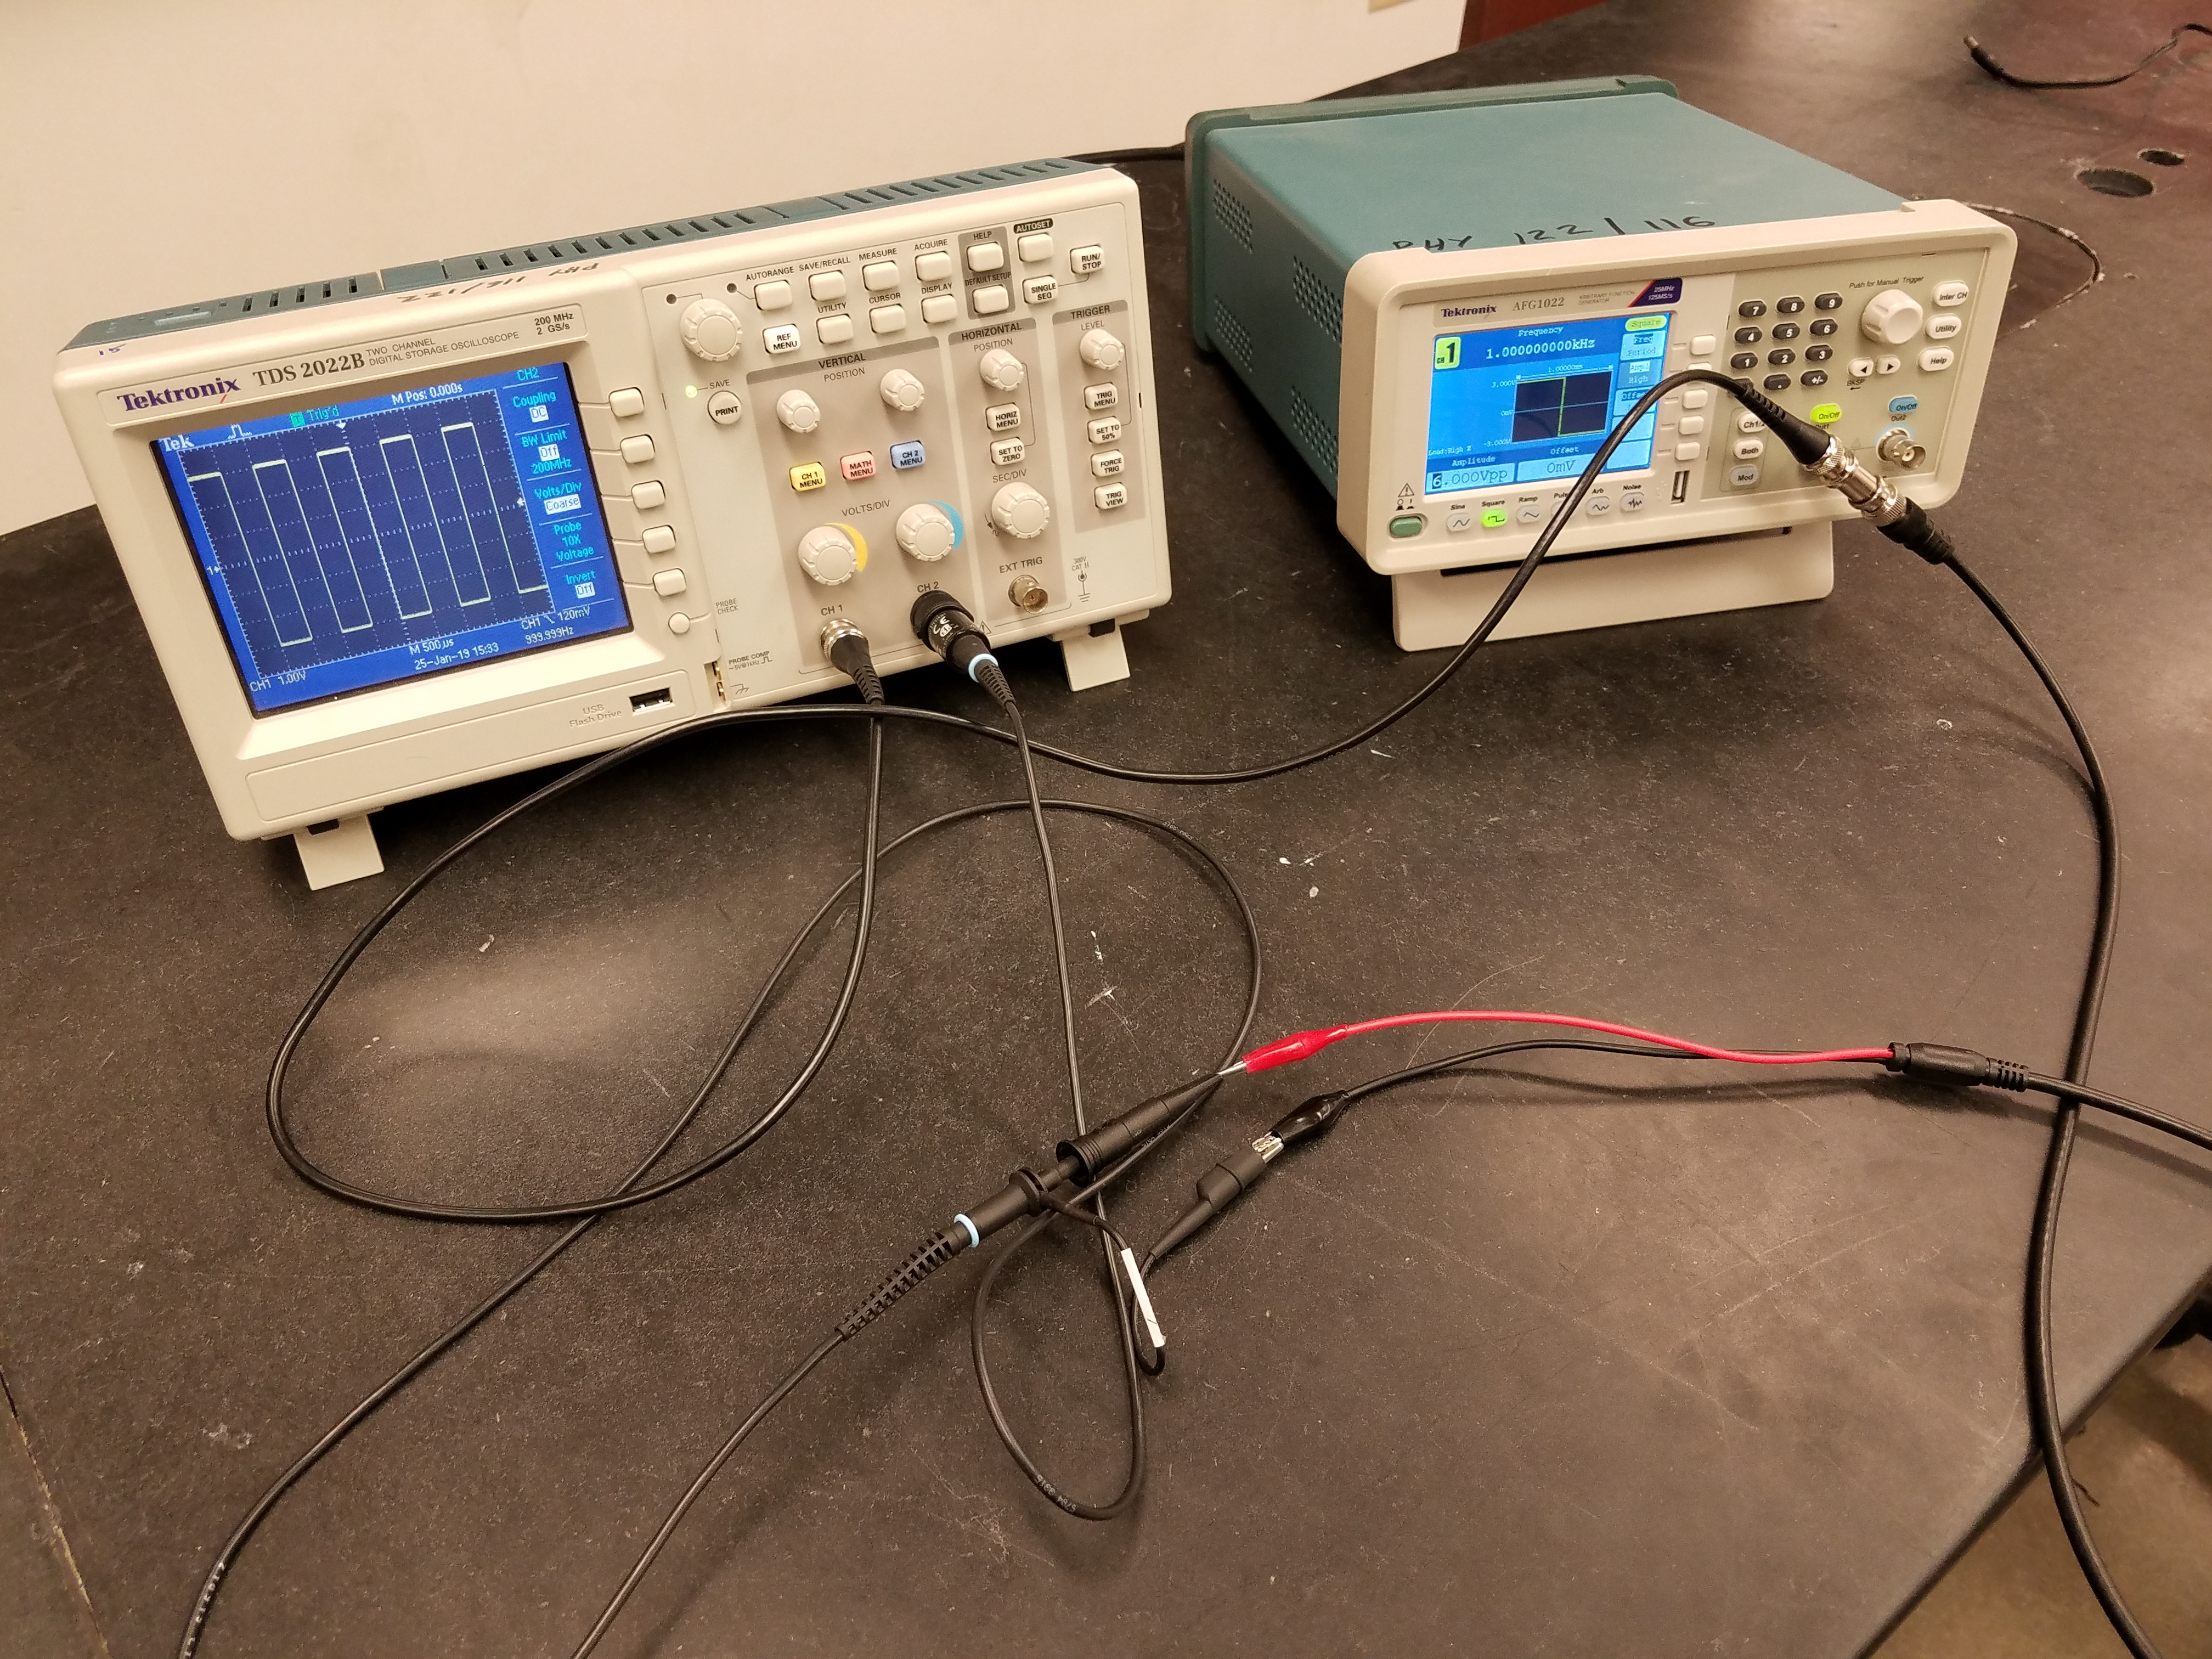
\includegraphics[height=0.30\textheight]{figs/labs/transients/probe_setup.jpg}};
         \node[left](X) at (-1.0,4.0) {Probe Tip}; \draw (X.east) --
         (5.0,2.4); \node[left](X) at (-1.0,3.0) {Ground Clip}; \draw
         (X.east) -- (5.4,2.2); \node[right](X) at (10.0,5.0) {BNC
           Tee}; \draw (X.west) -- (8.0,5.2); \node[right](X) at
         (10.0,4.0) {Alligator pair}; \draw (X.west) -- (6.5,2.8);
\end{tikzpicture}
\caption{A setup for connecting the scope probe directly to the output of the function generator.}
\label{fig:probe_setup}
\end{center}
\end{figure}

Install an oscilloscope probe at Channel 2 of your scope (see
Fig~\ref{fig:probe}).  Some probes in the lab have the ability to
switch between attenuation factors near the probe tip.  If you have
such a probe, select the 10X setting.  The remaining probes have a
fixed attenuation of 10X.

So far, we haven't had to worry about proper grounding procedure,
because this is automatically handled by the BNC cable.  Your scope
probe has two main parts, the larger probe tip, which slides to reveal
a hook which can be attached to wires and components in your circuit,
and a short lead ending with a black alligator clip called the
``Grounding clip''.  Handheld devices like your DMM have no connection
to earth ground.  The voltage reference point at the Common terminal
can be connected anywhere you would like in a circuit.  Your scope is
quite different!  It plugs into a wall outlet for power and is
referenced to earth ground.  To provide a scope which is both safe and
cost effective, most scopes are limited to making measurements which
are referenced to ground when using ordinary probes.  The ground clip
of your scope can only be connected to earth ground.  If you connect
it anywhere else in your circuit, that part of your circuit will be
short-circuited to ground.

For now, connect the probe directly to the output of the function
generator.  Your function generator is also referenced to earth
ground.  In particular for this setup, the black alligator clip is
earth ground.  Connect the black clip from the function generator to
the grounding clip for the scope probe.  Next connect the scope probe
to the red alligator clip from the function generator.  You now have
two copies of the function generator output being sent to the scope.
One directly through the BNC cable, and one through a 10X attenuation
scope probe.

Adjust your scope to view the function generator output as measured by
Trigger 1.  Set the voltage scale as large as possible while observing
the entire wave form.  Leave the timescale at the default setting of
$500~\mu s$ for now.  Check that trigger is on the Falling edge, as set
in the last section.  Set the trigger threshold near 0 volts.
You should observe that the position of the waveform does not vary
much with trigger threshold: the steep falling edge of the square wave
function gives us a solid reference point for defining $t=0$ in the
measurements that follow.

Now enable Channel 2 on your scope. Adjust all the necessary settings
for Channel 2 so that it produces an identical copy of Channel 1.  Too
see both channels at the same time, you'll have to move the vertical
position of Channel 1 slightly.  Closed loop tests like this are the
way experienced scientists and engineers always start.  It allows you
to setup your signal generator and scope properly, without adding the
complexity of the circuit you are working on.  In general, avoiding
confusion by taking small incremental steps is the fastest, most
reliable way to proceed in lab.

\begin{figure}[htbp]
\begin{center}
\begin{tabular}{cc}
\begin{circuitikz}[line width=1pt]
\draw (0,0) to[square voltage source,bipoles/length=1.5cm] ++(0,4.0) to[short] ++(2.0,0)
to[R,-*] ++(0,-2.0) coordinate(X) to[short,*-o] ++(1.0,0) node[right]{A};
\draw (X) to[C,-*] ++(0,-2.0) coordinate(X) to[short,-o] ++(1.0,0) node[right]{B};
\draw (X) to[short,-*] ++(-2.0,0) node[ground,yscale=2.0]{};
\end{circuitikz}  &
\begin{circuitikz}[line width=1pt]
\draw (0,0) to[square voltage source,bipoles/length=1.5cm] ++(0,4.0) to[short] ++(2.0,0)
to[R,-*] ++(0,-2.0) coordinate(X) to[short,*-o] ++(1.0,0) node[right]{A};
\draw (X) to[L,-*] ++(0,-2.0) coordinate(X) to[short,-o] ++(1.0,0) node[right]{B};
\draw (X) to[short,-*] ++(-2.0,0) node[ground,yscale=2.0]{};
\end{circuitikz}  \\
(a) & (b) \\
\end{tabular}
\caption{A function generator driving an (a) RC circuit, and (b) RL circuit.}
\label{fig:rlc-circuits}
\end{center}
\end{figure}

Select a $C=10~\rm nF$ capacitor and an $R=10~\rm k\Omega$.

\begin{measurement}
Using the given values of resistor and capacitor, calculate and record
in your logbook the time constant of the RC circuit.  Using your DMM,
measure and record the actual resistance and capacitance of your
components before installing them.
\end{measurement}

Construct the circuit in Fig.~\ref{fig:rlc-circuits}a on your
breadboard, as shown in Fig.~\ref{fig:rc_setup}a.  Your function
generator acts as the square wave voltage source.  Recall that the
black alligator clip is earth ground.  The red alligator clip is the
square wave output relative to earth ground, and corresponds to the
upper terminal of the voltage source in the diagram.  The only valid
place to connect the grounding clip of your scope probe is to earth
ground, so connect that to point B in your circuit.  Connect the scope
probe tip to point A.  As shown in the Fig.~\ref{fig:rc_setup}b, each
time the square wave changes polarity, the capacitor begins charging
or discharging until it reaches equilibrium with the new voltage,
revealing the characteristic exponential transient response.

\begin{figure}[htbp]
\begin{center}
\begin{tabular}{cc}
\includegraphics[width=0.45\textwidth]{figs/labs/transients/rc_setup.jpg} &
\includegraphics[width=0.45\textwidth]{figs/labs/transients/rc_trace.jpg} \\
(a) & (b) \\
\end{tabular}
\caption{Setup for the (a) RC circuit measurement, and (b) example scope trace showing exponential curve.}
\label{fig:rc_setup}
\end{center}
\end{figure}

\begin{figure}[htbp]
\begin{center}
\begin{tabular}{cc}
\includegraphics[width=0.45\textwidth]{figs/labs/transients/rc_cursor.jpg} &
\includegraphics[width=0.45\textwidth]{figs/labs/transients/rc_falltime.jpg} \\
(a) & (b) \\
\end{tabular}
\caption{Scope traces showing (a) use of cursor to measure the waveform at $t=124~\rm \mu s$ and $V=-1.20~\rm V$, (b) use of the built in fall time measurement.}
\label{fig:cursor_falltime}
\end{center}
\end{figure}

Now adjust the timescale to zoom in on the exponential decay portion
of the curve, making sure to keep the trigger position at the left
side of the display, as shown in Fig.~\ref{fig:cursor_falltime}a.
Press the Cursor button, then set Type to Time, and Source to CH2.
This feature allows you to make measurements of different points along
the curve.  Leave Cursor 1 located at $t=0$.  Highlight Cursor 2, by
pressing the corresponding menu button, and adjust it's position using
the multipurpose knob.  Now you can make accurate measurements of the
waveform by reading off the voltage and time at anywhere that you
place the cursor.  

\begin{measurement}
Record one measurement every $\sim 25~\rm \mu s$ starting from
$t=0~\mu s$ to $400~\rm \mu s$.  (Recall that when making measurements
at target values, you need not hit the target value exactly, simply
record the actual position at which you made your measurement.) Record
a rough sketch of your waveform.
\end{measurement}

For an exponential decay with time constant $\tau$, the rise-time (or fall-time),
when defined as the time interval between $10\%$ and $90\%$ values, is
given by:
\begin{displaymath}
t_{90} = {\rm ln}(9) \; \tau \sim 2.2 \; \tau
\end{displaymath}

\begin{measurement}
Your scope can also directly measure the fall time of a waveform.  For
an accurate measurement, setup the scope so that one complete falling
edge is on screen, as shown in Fig.~\ref{fig:cursor_falltime}b.  Press
Measure and then set source to CH2 and Type to ``Fall Time''. You
might see this value fluctuating.  In such circumstances, it's a good
practice to record 3-5 different measurements to help intepret your
results later.

The manufacturer does not specify the accuracy of the fall-time
measurement, but from other specifications we can reasonably infer an
accuracy of about $3\%$ for the setting used in this lab.  The values of $R$ and $C$ measured with your DMM are much more precisely known than $3\%$.  Does your predicted time-constant based on the measured values of $R$ and $C$ agree with the measured fall time?
\end{measurement}

This is a \textbf{sign-off point} for this lab.

\begin{plot}
Plot your collected $RC$ circuit voltage-versus-time data as discrete
data points.  On the same plot, compare the data to the expected
exponential decay function as a continuous curve, using the $RC$ time
constant calculated from the measured values of $R$ and $C$.  Make
sure to have appropriate axis labels and a legend indicating ``Data''
and ``Prediction''.
\end{plot}
  
\section{Transient response of an RL circuit}

Not everyone will have time to finish this entire section, do your
best with your available time.

\begin{measurement}
Calculate the inductance of a solenoid with N=20 turns, length
$\ell=4~\rm cm$, a radius of $1~\rm cm^2$ using the formula:
\begin{displaymath}
L = \frac{\mu_0 N^2 A}{\ell}
\end{displaymath}
where $A$ is the cross-sectional area and $\mu_0 = 1.257 \times 10^{-6}~\rm H/m$.
\end{measurement}

\begin{measurement}
Wrap an inductor around the provided wooden dowel. Estimate it's
inductance by modifying your calculation above accordingly and record
the value in your logbook.
\end{measurement}

Obtain a $R=47~\rm \Omega$ resistor.
\begin{measurement}
Using your DMM, measure and record the resistance of your resistor.
\end{measurement}

Turn down the supply to $2.5~\rm V$ peak-to-peak.  Build the
circuit in Fig.~\ref{fig:rlc-circuits}b using your homemade inductor
and your resistor.

\begin{measurement}
Using your digital scope, measure the fall-time of your RL circuit and
use it to determine a measured value for the inductance.  Calculate
the inductance of your coil homemade coil and compare to your
theoretical estimate.  Briefly explain your result in your logbook
\end{measurement}

This is an additional \textbf{sign-off point} for this lab.

\chapter{Passive Filters and Resonance}

\begin{figure}[htbp]
\begin{center}
\begin{tabular}{c@{\hskip 2cm}c}

\begin{circuitikz}[line width=1pt]
\draw (0,0) to[sinusoidal voltage source,bipoles/length=1.5cm] ++(0,4.0) to[short] ++(2.0,0)
to[R,-*] ++(0,-2.0) coordinate(X) to[short,*-o] ++(1.0,0) node[right]{A};
\draw (X) to[C,-*] ++(0,-2.0) coordinate(X) to[short,-o] ++(1.0,0) node[right]{B};
\draw (X) to[short,-*] ++(-2.0,0) node[ground,yscale=2.0]{};
\end{circuitikz}  &

\begin{circuitikz}[line width=1pt]
\draw (0,0) to[sinusoidal voltage source,bipoles/length=1.5cm] ++(0,4.0) to[short] ++(2.0,0)
to[R,-*] ++(0,-2.0) coordinate(X) to[short,*-o] ++(1.0,0) node[right]{A};
\draw (X) to[C,-*] ++(0,-2.0) coordinate(X) to[short,-o] ++(1.0,0) node[right]{B};
\draw (X) to[short,-*] ++(-2.0,0) node[ground,yscale=2.0]{};
\end{circuitikz}  \\


(a) & (b) \\
\end{tabular}
\caption{A function generator driving a resistor.}
\label{fig:mycirc}
\end{center}
\end{figure}


\section{Resonant Band-pass Filter}

\begin{figure}[htbp]
\begin{center}

\begin{circuitikz}[line width=1pt]
\draw (0,0) to[sinusoidal voltage source,bipoles/length=1.5cm] ++(0,3.0) 
to[R,-*] ++(2.0,0) coordinate(X) to[short,*-*] ++(1.5,0) coordinate(Y) to[short,-o] ++(1.0,0) node[right]{A};
\draw (X) to[C,-*] ++(0,-3.0)  to[short,-*] ++(-2.0,0) node[ground,yscale=2.0]{};
\draw (Y) to[L,-*] ++(0,-3.0)  coordinate(X) to[short,-*] ++(-1.5,0);
\draw (X) to[short,-o] ++(1.0,0) node[right]{B};
\end{circuitikz}  
\caption{A function generator driving a resistor.}
\label{fig:mycirc}
\end{center}
\end{figure}


\section{Pre-lab Calculations}

\noindent
1) Calculate the crossover frequency (aka the $-3~\rm dB$ point) for the RC filter shown in Fig.~\ref{fig:lowpass}a. \\ \vskip 0.25cm

\noindent
2) Using the formula derived in lecture, calculate the resonant angular frequency $\omega_0$ and resonant frequency $f_0$ of the resonant circuit in Fig.~\ref{fig:rlc}.  {\em A very common mistake is to mixup frequency and angular frequency in the lab.} \\ \vskip 0.25cm

\noindent
3) Using the formula derived in lecture, calculate the $Q$-factor for the resonant circuit in Fig.~\ref{fig:rlc}.

\section{Introduction}

\begin{figure}[htbp]
\begin{center}
%\begin{tabular}{c@{\hskip 0.25in}c}
\begin{tabular}{cc}
\includegraphics[height=0.22\textheight]{figs/labs/filters/bode.pdf}
&
\includegraphics[height=0.22\textheight]{figs/labs/filters/phase.pdf} \\
(a) & (b) \\
\end{tabular}
\end{center}
\caption{\label{fig:bode} Bode plots for highpass and lowpass filters showing the (a) gain on a dB scale, and (b) phase, both as a function of the ratio of frequency $f$ to the crossover frequency $f_0$ on a log scale.}
\end{figure}

In this lab, you will build and measure the performance of a lowpass and a highpass $RC$ filter, and produce Bode plots to compare your circuit with the impedance model derived in class and shown in Fig.~\ref{fig:bode}.  You will build an $RLC$ bandpass filter, determine its resonant frequency and quality factor, and see how limitations from non-ideal components dramatically affect the performance of real circuits.

\section{Lowpass Filters}


\noindent
You'll be using two scope probes in this lab, and some care must be taken when using their grounding clips.  The only place you may connect the grounding clip from a scope probe is to the ground in your circuit. For a battery powered device not connected to earth ground, you could choose this ground point to be anywhere, as long as it was consistent for both scope channels.  But in our circuit, the function generator is already referenced to earth ground, and therefore the only possible choice for the ground location is at the negative terminal of the function generator, as already shown in the circuit diagrams.  Always remember that when you connect a scope probe grounding clip, you short that point to earth ground through the scope!  {\bf In these circuits, the only place you may attach a scope probe grounding clip is at the point $\boldmath P_1$, i.e. at the negative terminal of the function generator.}


\begin{figure}[htbp]
\begin{center}
\includegraphics[height=0.35\textheight]{figs/labs/filters/scope_gain.pdf}
\end{center}
\caption{\label{fig:scopegain} The gain and phase change measurement using an oscilloscope.
Here the gain is $1.4/2.0 = 0.7 \sim 1/\sqrt{2}$.  Later times appear toward the right, so the output is lagging the input, and therefore the phase shift is negative.  The size of the time offset is $25~\rm ms$ in a period of $200~\rm ms$ so the phase shift is $\phi = -\pi/4$.  This is what engineers like to call the $-3~\rm dB$ or even just the $3~\rm dB$ point, because $20 \log_{10} \sqrt{2} = 3.01$.  Just to confuse physicists!}
\end{figure}

We'll be measuring two potentials simultaneously for all of the filters in this lab.  The input voltage $V_{\rm in}$ is measured between ground at $P_1$ and the point $V_{\rm in}$ in the circuit.  This can be measured by using a ``BNC T" to connect both your scope and your circuit to the function generator output.  Alternatively, use a scope probe with the grounding clip at $P_1$ and the the probe tip at $V_{\rm in}$.  The output voltage $V_{\rm out}$ is measured using a scope probe with the grounding clip at $P_1$ and the probe tip at $V_{\rm out}$.  We will be measuring the voltage gain $G = V_{\rm out} / V_{\rm in}$ and the phase shift $\phi$ of $V_{\rm out}(t)$ relative to $V_{\rm in}(t)$. 

Build the circuit shown in Fig.~\ref{fig:lowpass}a using $R=1.5~\rm k \Omega$ and $C= 0.01~\rm \mu F$.   Use your function generator in AC mode with a peak-to-peak voltage of $4~\rm V$.   Either put the function generator in high impedance output mode, or select the $50~\rm \Omega$ output impedance and use a $50~\rm \Omega$ terminator.

Vary the frequency above and below the cross-over frequency which you calculated, and verify the behavior qualitatively before proceeding with the data taking.  As this is a low-pass filter, you should expect to see the gain $V_{\rm out}/V_{\rm in} = 1/\sqrt{2}$ with a phase shift $\phi = -\pi/4$ at the crossover frequency.  An example measurement at the crossover frequency is shown in Fig.~\ref{fig:scopegain}.  Below this frequency you should approach unit gain, and above this frequency the gain should fall rapidly.  

To make these measurements accurately, you should first confirm that both channel 1 and channel 2 on your scope are vertically aligned with the $x$-axis (i.e. the thick central horizontal line on the display), which you do by temporarily setting the coupling of each channel to ground (i.e. V=0) and adjusting the horizontal offset as needed.  Next, adjust the trigger setting to trigger on the rising edge of $V_{\rm in}$ and set the trigger threshold at zero.  Learn to use your scope's cursor function.  For instance, when making the phase shift measurement, you would place the reference cursor at the point where 
$V_{\rm in}$ crosses zero with positive slope (the trigger point) and measure the point where $V_{\rm out}$ crosses zero with positive slope using the cursor.

Once you are certain your circuit is working properly and you scope is configured to measure the magnitude and gain accurately, take measurements at 9 different frequencies, chosen to cover four decades of frequency range and uniform in the log of the frequency:
\begin{displaymath}
f=\{f_0/100, f_0/30, f_0/10, f_0/3,f_0, 3f_0, 10f_0, 30f_0, 100f_0\}
\end{displaymath}
where $f_0$ is the cross-over frequency.  At each frequency, you will measure the gain:  $G = V_{\rm out} / V_{\rm in}$ and the phase shift $\phi$ of $V_{\rm out}$ relative to $V_{\rm in}$.  

If you prefer, you can use your scope's measurement features (which include a phase measurement) after making a few measurements from the wave form as described above.  When using automated features, it is usually a good idea to make a few manual measurements first to make sure you are measuring what you think you are.

\section{Highpass Filter}

Using the same components as in the previous section, build the high-pass filter of Fig.~\ref{fig:highpass}a.  Verify the operation of the circuit at the crossover frequency (aka 3 db point) where we expect the gain to be $1/\sqrt{2}$ as before but the phase shift to be {\em positive} $\phi = \pi/4$.

As in the preceding section, measure the magnitude and phase of the gain as a function of frequency, but to save time, you may omit some measurements:
\begin{displaymath}
f=\{f_0/10, f_0/3,f_0, 3f_0, 10f_0\}
\end{displaymath}
where $f_0$ is the crossover frequency.

\section{Bandpass Filter}


In lecture, we showed that the resonant angular frequency of an RLC bandpass filter is given by
\begin{equation}
\omega_0 = \frac{1}{\sqrt{LC}}. 
\end{equation}
At this frequency, the RLC resonant circuit has unit gain and no phase shift.  As the frequency moves away from the resonant frequency, the gain drops.  We define two points $\omega_+$ and $\omega_-$ as the two frequencies, one above and one below $\omega_0$, at which the gain drops below $1/\sqrt{2}$.  These are the two $-3~\rm dB$ points which define the bandwidth of the system.  We define the quality of the resonance by the ratio of resonant frequency to this bandwidth:
\begin{displaymath}
Q = \frac{\omega_0}{\omega_+ - \omega_-} = \frac{f_0}{f_+-f_-}
\end{displaymath}
For the RLC resonant circuit, we showed in lecture that:
\begin{equation}
Q = \omega_0 RC
\end{equation}

Build the circuit in Fig.~\ref{fig:rlc} using $R=1~{\rm k \Omega}$ , $C=4.7~\rm{\mu F}$, and $L=150~\rm \mu H$.
Set the frequency of the function generator to $f_0 = \omega_0/2\pi$  and the peak-to-peak voltage $10~\rm V$.

\begin{figure}[htbp]
\begin{center}
\includegraphics[height=0.35\textheight]{figs/labs/filters/scope_xy.pdf}
\end{center}
\caption{\label{fig:scopexy} Example scope traces in XY display mode for a relative phase $\phi=\pi/2$, 
$\phi=\pi/4$, and $\phi=0$.  It is easy, accurate, and somehow deeply satisfying to tune the frequency until the ellipse collapses into itself, forming a line.}
\end{figure}

We'll determine the resonant frequency using a trick.  During normal use, your oscilloscope displays the voltage of each channel versus time.  But there is an ``XY" mode available under the display options.  In this mode, the scope displays the voltage of channel one versus the voltage of channel two.  When in XY mode, two out-of-phase signals yield an ellipse.  But, as shown in Fig.~\ref{fig:scopexy} when both channels are perfectly in phase, the ellipse collapses to make a diagonal line.  You can set you scope in XY mode and adjust the frequency until the ellipse collapses to quickly and accurately find the resonance frequency.

One you determine the resonant frequency, switch back to the normal display mode and determine the bandwidth.  The easiest way to obtain this is to use the curser to measure the peak voltage of your output signal.  Multiply this by a factor of $1/\sqrt{2} = 0.7$ to determine the $-3~\rm dB$ amplitude and set the second curser at this value.  Now adjust the frequency above and below the resonant frequency and note at which frequencies the amplitude drops below this line.  The difference between these two points is your $f_+$ and $f_-$.

From your measurement of $f_0$, $f_+$, and $f_-$ you can calculate the measured $Q$-factor of your circuit.  It will be quite different than what you calculated in pre-lab! 

\section{Degradation of the $Q$-factor}

The $Q$-factor that you measured in the previous section is significantly lower than the theoretical $Q$-factor for the circuit in Fig.~\ref{fig:rlc}.  In fact, the inductor is non-ideal in a number of ways.  In this case, there is a parasitic parallel resistance that makes the circuit effectively that of Fig.~\ref{fig:rlcpar}.  The resistance $R_{\rm P}$ is already present (unfortunately!) in your circuit.  

It turns out that the $Q$ factor is degraded in this case to the value:
\begin{equation}
Q = \omega_0 C \frac{R R_{\rm P}}{R+R_{\rm P}}
\end{equation}

To determine $R_P$, note that at the resonant frequency, the parallel impedance of $L$ and $C$ are infinite, and so can be treated as open circuits.  The circuit becomes a voltage divider with two resistors $R$ and $R_P$.  By measuring the gain $V_{\rm out}/V_{\rm in}$ at the resonant frequency, you should be able to determine $R_P$, and correct your gain calculation accordingly.  Now how does your calculated $Q$-factor compare with what you measured?


\section{Lab Report}

Your report should include all of your calculations, and the plotted response of your lowpass and highpass circuits as in Fig.~\ref{fig:bode}.  In addition to the gain in dB, also produce a plot with $V_{\rm out}/V_{\rm in}$.  Answer all questions in the text.

Notice that the difference between the RC highpass and lowpass filter just amounts to which component we measure the voltage $V_{\rm out}$ across.  Therefore, one might reasonably expect the crossing point of the Bode plots to occur where $V_{\rm out}/V_{\rm in} = 0.5$, but, in fact, it occurs at the 3~dB point where $V_{\rm out}/V_{\rm in} = 0.7$.  How is this be possible?  Does the voltage across the resistor plus the voltage across the capacitor add to 1.4 times the input voltage?!

 


\chapter{Lissajous Figures and Resonance}


\section{Introduction}

In this lab, you'll view Lissajous curves in 2-D using the $X$-$Y$ mode of your scope and reproduce the same curves using parameterized equations in Scientific Python. You will also  build and measure the performance of a $RLC$ band-pass filter and determine its resonant frequency and quality (Q) factor. For this lab there are both logbook and jupyter notebook entries.

\section{Lissajous Figures}

\begin{figure}[htbp]
\begin{center}
\begin{tabular}{cc}
\includegraphics[width=0.45\textwidth]{figs/labs/lissajous/scope_lissajous.jpg} & 
\includegraphics[width=0.45\textwidth]{figs/labs/lissajous/scope_crown.jpg} \\
(a) & (b) \\
\end{tabular}
\caption{Scope traces from Lissajous figures from settings for (a) start, and (b) crown.}
\label{fig:tracelissajous}
\end{center}
\end{figure}
Lissajous figures are the graph of system of two parameterized functions:
\begin{eqnarray*}
x &=& A_1 \sin(2 \pi f_1 t + \delta) \\
y &=& A_2 \sin(2 \pi f_2 t) 
\end{eqnarray*}
which produces a closed loop if the ratio $A_1 / A_2$ is rational.  The appearance of the figure is of a 3 dimensional knot with the viewing angle determined by the parameter $\delta$.  Two examples are shown in Fig.~\ref{fig:tracelissajous}.

To produce these figures on your scope, we'll need to use two
channels.  To begin, enable the output of both Channel 1 and Channel 2
on your function generator, and set them both to produce sine waves
with amplitude $3~\rm V$ peak-to-peak.  Adjust the frequency of
channel 1 to $2~\rm kHz$ and the channel 2 to $3~\rm kHz$.  Note that
you can switch between the Channel 1 and Channel 2 parameter menus on the function generator
with the button labeled ``Ch1/2''.

\begin{figure}[htbp]
\begin{center}
\includegraphics[width=0.45\textwidth]{figs/labs/lissajous/two_sine.jpg} 
\caption{Correctly scaled scope output.}
\label{fig:twosine}
\end{center}
\end{figure}

On your scope, switch to the Channel 2 parameter menu by pressing the
blue button labeled ``2''.  Set the coupling of Channel 2 to AC, and
probe attenuation to 1x, just as you did previously for Channel 1.
Next adjust the voltage scales of each channel to $500~\rm mV$ and set
the common time scale to something appropriate, so that you can view
both Sine waves on the scope display.  As shown in Fig.~\ref{fig:twosine},
you will see two versions of the Channel 2 output, inverted with
respect to each other, because the frequency of Channel 2 is 1.5 times
the frequency of Channel 1. You can check this but changing slightly the frequency of 
Channel 2 but return it to prescribe values to continue with the lab.

The relative phase between the two output channels of your function
generator shifts whenever you adjust the frequency of one of the
signals.  For consistent results with offline plots and the scope
traces shown here, you'll need to align the phase of the two channels
every time you adjust the frequency on the function generator:
\begin{displaymath}
\rm Inter Ch button \to AlignPhase.
\end{displaymath}

Usually, scopes are used to display the inputs as a function of time.
In this case, the voltage level is along the $y$-axis, and time is the
$x$-axis.  This mode is called YT mode.  Occasionally, however, it is
useful to display things in XY mode.  In this mode, the $x$-axis is
used for the voltage of Channel 1 and the $y$-axis is used for the
voltage of Channel 2.  Each point on the curve represents a particular
point in time.  Switch to XY mode by pressing the Display button and
then pressing the button next to the Format menu item until the mode
is XY.  You should reproduce Fig.~\ref{fig:tracelissajous}a
exactly.  If not, check that you have aligned the phase as described
above and that frequencies are set correctly as in Table.

\begin{table}
\begin{center}
\caption{Settings for various Lissajous figures.}
\label{tbl:lissajous}
\begin{tabular}{llll}
pattern & $f_1~\rm(kHz)$ & $f_2~\rm(kHz)$ & $\delta_1$ \\
start & 2 & 3 & 0 \\
fish & 2 & 3 & $135^\circ$ \\
parabola & 1 & 2 & $45^\circ$ \\
lace & 13 & 12 & 0 \\
crown & $1~\rm kHz$ & $4~\rm kHz$ & 0 \\
\end{tabular}
\end{center}
\end{table}

\begin{plot} Adjust the phase of Channel 2, under menu item StartPhase, until the
pattern collapses into a Fish pattern (or greek letter $\alpha$) at
135 degrees. Make sure that there is a date printed on the screen of your scope trace.  Save a scope trace by inserting your USB drive into the
scope and pressing the Save button (it takes few seconds to save).  \end{plot}

 \begin{plot}Then produce the parabola pattern  according to the settings in Table~\ref{tbl:lissajous}, saving a scope
trace.  Remember to align the phase each time you change the frequency.\end{plot}
\begin{plot} Produce lace pattern and save a scope trace. \end{plot}

\begin{plot} Next, produce the crown pattern, shown in Fig.~\ref{fig:tracelissajous}b.
For the right proportions, adjust the amplitude of
Channel 2 to $1~\rm V$ peak-to-peak, leaving Channel 1 at $3~\rm V$
peak-to-peak.  Notice that as you adjust the phase of Channel 1, the
crown appears to rotate.  Adjust the frequency of Channel 2 to
$4.0002~\rm kHz$.  The crown should now appear to rotate constantly at
low speed.  \end{plot}

\noindent
Include your saved scope traces of Lissajous figures in the python notebook. Provide a full label for each plot which describes all the relevant information. 

\section{Band-pass Filter}



\begin{figure}[htbp]
\begin{center}
\begin{circuitikz}[line width=1pt]
\draw (0,0) to[sinusoidal voltage source,bipoles/length=1.5cm] ++(0,3.0) 
to[R,-*,l_=$R_1$] ++(2.0,0) coordinate(X) to[short,*-*] ++(1.5,0) coordinate(Y) to[short,-o] ++(1.0,0) node[right]{B};
\draw (X) to[C,-*,l=$C_1$] ++(0,-3.0)  to[short,-*] ++(-2.0,0) node[ground,yscale=2.0]{};
\draw (Y) to[L,-*,l=$L_1$] ++(0,-3.0)  coordinate(X) to[short,-*] ++(-1.5,0);
\draw (X) to[short,-o] ++(1.0,0) node[right]{A};
\end{circuitikz}  
\caption{Circuit diagram for RLC band-pass filter.}
\label{fig:rlc_circuit}
\end{center}
\end{figure}


%\begin{figure}[htbp]
%\begin{center}
%%\begin{tabular}{c@{\hskip 0.25in}c}
%\begin{tabular}{cc}
%\includegraphics[height=0.22\textheight]{figs/labs/filters/rcgaindb.pdf}
%&
%\includegraphics[height=0.22\textheight]{figs/labs/filters/rcphase.pdf} \\
%(a) & (b) \\
%\end{tabular}
%\end{center}
%\caption{\label{fig:bode} Bode plots for band-pass filter showing the (a) gain on a dB scale, and (b) phase, both as a function of the ratio of frequency $f$ to the crossover frequency $f_0$ on a log scale.}
%\end{figure}

%
%\begin{measurement} Calculate the resonant frequency:
%\begin{equation}
%f_0 = \frac{1}{2\pi \sqrt{LC}}. 
%\end{equation}
%of the resonant circuit in Fig.~\ref{fig:rlc_circuit}
%for $R_1=1.5~\rm k\Omega$, $C_1=10~\rm nF$, and $L_1 = 1~\rm mH$.
%\end{measurement}


%In lecture, we showed that the resonant angular frequency of an RLC
%band-pass filter is given by
%\begin{equation}
%\omega_0 = \frac{1}{\sqrt{LC}}. 
%\end{equation}
%At this frequency, the RLC resonant circuit has unit gain and no phase
%shift.  As the frequency moves away from the resonant frequency, the
%gain drops.  We define two points $\omega_+$ and $\omega_-$ as the two
%frequencies, one above and one below $\omega_0$, at which the gain
%drops below $1/\sqrt{2}$.  These are the two $-3~\rm dB$ points which
%define the bandwidth of the system.  We define the quality of the
%resonance by the ratio of resonant frequency to this bandwidth:
%
%\begin{displaymath}
%Q = \frac{\omega_0}{\omega_+ - \omega_-} = \frac{f_0}{f_+-f_-}
%\end{displaymath}

%For the RLC resonant circuit, we showed in lecture that:
%\begin{equation}
%Q = \omega_0 RC
%\end{equation}

\noindent Build the circuit in Fig.~\ref{fig:rlc_circuit} using $R=1.5~{\rm k \Omega}$ ,
$C=10~\rm{n F}$, and $L=1~\rm mH$. 
\begin{measurement} Using your DMM, measure and record
the actual resistance and capacitance of your components before
installing them. Use an LCR meter (BK Precision 878B)  to measure the actual inductance of the inductor and record it. Sketch the setup in your logbook.
Calculate $f_0$ using the measured values of your components. 
\begin{equation}
f_0 = \frac{1}{2\pi \sqrt{LC}}. 
\end{equation}
\end{measurement} 

\noindent Set the frequency of the function generator to $f_0$ and the peak-to-peak
voltage to $4~\rm V$.

\begin{figure}[htbp]
\begin{center}
\includegraphics[width=0.50\textwidth]{figs/labs/filters/scope_xy.pdf}
\end{center}
\caption{\label{fig:scopexy} 
Expected scope traces in $XY$ display mode for a relative phase $\phi=\pi/2$, 
$\phi=\pi/4$, and $\phi=0$.  It is easy, accurate, and somehow deeply satisfying to tune the frequency until the ellipse collapses into itself, forming a line.}
\end{figure}

We'll measure the actual resonant frequency using a trick: an $XY$ mode of the scope.  
%During normal use, your oscilloscope displays the voltage of each channel versus
%time.  But there is an $XY$ mode available under the display options.
%In this mode, the scope displays the voltage of channel one versus the
%voltage of channel two.  
When in $XY$ mode, two out-of-phase signals
yield an ellipse.  But, as shown in Fig.~\ref{fig:scopexy} when both
channels are perfectly in phase, the ellipse collapses to make a
diagonal line. 
\begin{measurement} You can set you scope in XY mode and adjust the
frequency until the ellipse collapses to quickly and accurately find
the resonance frequency. Record the value in your logbook. Add comment in your logbook about how this measurement  compares to the calculated resonance frequency.
\end{measurement}
\begin{figure}[htbp]
\begin{center}
\includegraphics[width=0.45\textwidth]{figs/labs/filters/qscope.jpg}
\end{center}
\caption{\label{fig:qscope} Set Cursor 1 to the peak of Signal 2 at the resonant frequency, then set Cursor 2 to this value times $1/\sqrt{2}$.  The frequencies $f_+$ and $f_-$ can be determined by adjusting the frequency until the output amplitude reaches the level of Cursor 2, as shown here for $f_-$.
}
\end{figure}


\begin{measurement} One you determine the resonant frequency, switch back to the normal
display mode and determine the bandwidth.  The easiest way to obtain
this is to use the cursors to measure the peak voltage of your output
signal.  Multiply this by a factor of $1/\sqrt{2}$ to determine
the $-3~\rm dB$ amplitude and set the second cursor at this value, as
shown in Fig.~\ref{fig:qscope}.  Now adjust the frequency above and
below the resonant frequency and record at which frequencies the
amplitude reaches this line. Calculate the bandwidth and record it in your logbook.
\end{measurement}

\begin{measurement} From your measurement of $f_0$, $f_+$, and $f_-$ calculate the
measured $Q$-factor of your circuit. Record this value in your logbook. 
\end{measurement}


\noindent
This is a \textbf{sign-off point} for this lab. 

\section{Lissajous Figures Analysis}

\begin{plot} Reproduce fish pattern using scientific
python to draw the parameterized shape.  For
example, see Fig.~\ref{fig:pythonlissajous}. \end{plot}
\begin{plot} Reproduce  parabola pattern. \end{plot} 
\begin{plot} Reproduce crown pattern. \end{plot}

One way to approach this problem is to set the period to $1~\mu s$.
The functions should be evaluated at 1000 discrete times within the
interval from 0 to $1~\mu s$.
\begin{verbatim}
     t = np.linspace(0,1,num=1000)
\end{verbatim}
Define a fundamental angular frequency $\omega_0 = 2 \pi~\rm kHz$:
\begin{verbatim}
     w = 2*np.pi
\end{verbatim}
With these definitions, we would define:
\begin{verbatim}
     x = np.sin(4*w*t)
\end{verbatim}
to obtain $x$ points corresponding to $f=4~\rm kHz$ sine function.

When plotting your curves, use:
\begin{verbatim}
       plt.axis('equal')
\end{verbatim}
to keep the unit aspect ratio used by your scope.
%You can display your scope traces in python using the Image library like this:
%\begin{verbatim}
%       import Image
%
%       image = Image.open('myscope.jpg')
%       image.show()
%\end{verbatim}

\begin{figure}[htbp]
\begin{center}
\includegraphics[width=0.45\textwidth]{figs/labs/lissajous/pythonlissajous.pdf} 
\caption{Lissajous curve constructed using Scientific Python corresponding to the scope trace in Fig.~\ref{fig:tracelissajous}a.}
\label{fig:pythonlissajous}
\end{center}
\end{figure}

\chapter{Probability Distributions}

\section{Introduction}

In this lab, you will create your own simulation of a binomial
process, and compare the results of your simulation with the PDFs for
the binomial, Poisson, and Gaussian processes in the appropriate
limits.

This lab includes a number of code snippets to illustrate the ideas
that are being discussed.  However, the entire source listing is not
available to you, as this would amount to giving away the answer.  You
will also notice that most of the code snippets cannot be cut and
pasted.  This is all intentional.  The examples should help you
understand what you should do, but you will have to write your own
code.  {\bf Do not expect the code snippets as written to work for
your code without any modification... they are not supposed to!}

\section{Simulating the Binomial Process}

Your first task is to create a Monte Carlo simulation for a binomial
process.  The Monte Carlo method, named after the casino in Monaco, refers
to the repeated sampling of random variables to obtain numerical results.

Suppose one single experiment consists of $n_{\rm try}$ trials with a
probability $\epsilon$ of success.  The outcome of each experiment is
a single number from 0 to $n_{\rm try}$ reporting the number of the
$n_{\rm try}$ trials from that particular experiment which were
successful.  To study the distribution of outcomes, you will repeat the
experiment $n_{\rm exp}$ times.

There are libraries functions that will simulate this process for you,
but for this lab you will create your own simulation.  While
developing your code, start with a small test. For instance $n_{\rm
  try} = 3$ and $n_{\rm exp}=5$, as shown in the example below.
Implement your Monte Carlo simulation in the following manner:
\begin{itemize}
\item Create a 2-D array of shape $n_{\rm exp}$ by $n_{\rm try}$
  filled with random values chosen uniformly from 0 to 1.0:\\
\includegraphics[width=0.85\textwidth]{figs/labs/distributions/makearray.png} \\
This array associates a random value with each trial from each
experiment.  
\item Consider a trial successful if the randomly chosen value is less
  than $\epsilon$.  In this example, taking $\epsilon = 0.5$ and
  assuming 1 indicates success and 0 a failure, we obtain:
\begin{samepage}
\begin{verbatim}
[[1 1 0]
 [0 1 0]
 [0 1 1]
 [1 0 1]
 [1 0 0]]
\end{verbatim}
\end{samepage}
In the first simulated experiment, the first two trials were
successful and the last trial failed.  In the second experiment, the
first trial failed, the next trial was successful, and the last trial
failed.  And so on.

\item Next, count the number of trials that were successful in each experiment.  The result will be a 1-D array of length $n_{\rm exp}$.  Consider using the {\tt np.sum} function with the {\tt axis} parameter.  In this example, we obtain the array of outcomes $m$:
\begin{verbatim} 
[2 1 2 2 1]
\end{verbatim}
This is the outcome of our five simulated experiments.  The first
experiment has two out of three trials successful, the second
experiment had one out of three trials successful, and so on.
\end{itemize} 
Work through the example and make sure you see how each result follows
from the previous step.  Then implement and test your own version in
Scientific Python.  When validating a numerical calculation, think hard
about good test cases.  For instance, if you only test with the value
of $\epsilon = 0.5$, you won't catch a bug that mistakes success for
failure.  Try a few different test cases, with reasonably small values
for $n_{\rm try}$ and $n_{\rm exp}$ and check your numerical
simulation.  Boundaries often make a good check, for instance
$\epsilon = 0$ and $\epsilon = 1$.

Another effective validation strategy is to check known mathematical
relations using your simulation.  For instance, we know that the mean
value of a Binomial distribution is given by:
\begin{equation} \label{eqn:binom_mean}
\bar{m} = n_{\rm try} \cdot \epsilon
\end{equation}
and that the variance is given by:
\begin{equation} \label{eqn:binom_var}
\sigma^2 = n_{\rm try} \cdot \epsilon \, (1 - \epsilon)
\end{equation}
and so these predicted values, calculated from your parameters
$\epsilon$ and $n_{\rm try}$ can be compared to the mean and variance
of the outcome array $m$ from your simulation, calculated using the numpy functions {\tt np.mean} and {\tt np.var}.  A
comparison with $n_{\rm exp}=1000$, $n_{\rm try}=10$, and
$\epsilon=0.5$ should result in something like:\\
\includegraphics[width=0.85\textwidth]{figs/labs/distributions/validate.png}\\ 
Produce a large number of pseudo-experiments by setting $n_{\rm exp} =
1000$ and comment out any debugging print statements which will get
very long.  Pick five well chosen test cases with different values of
$n_{\rm try}$ and $\epsilon$ and compare the expected and simulated
mean and variances.  The simulated values will fluctuate by a
fractional amount $1/\sqrt{n_{\rm exp}}$.  So for $n_{\rm exp} =
1000$, we expect the expected and simulated values to agree within
about $3\%$.  If you increase to $n_{\rm exp} = 100000$, the agreement
should improve to better than $1\%$.  Be certain to record your test
cases and the results in your logbook.

\section{Histogram for the Binomial Process}

We use histograms to represent the distribution of numerical data.
Fill an output array $m$ with the results of $n_{\rm exp} = 1000$
experiments each consisting of $n_{\rm try}=10$ trials with success rate
$\epsilon=0.25$.  There are eleven possible outcomes for each of these
experiments: $0,1,2,\ldots,10$.  Construct a histogram from these 1000
outcomes using the {\tt np.histogram} function:\\
\includegraphics[width=0.85\textwidth]{figs/labs/distributions/makehist.png} \\
This calculates a histogram with eleven bins covering the range from
zero to eleven, and reports the number of outcomes from $m$ that occur
in each bin.  It returns two arrays, which we save as {\tt counts} and
{\tt bines}.  We interpret the outcome of the {\tt counts} array as follows:  60
experiments have zero successes, 164 experiments have one success, 281
experiments have two successes, and so on.  The exact values will vary
each time you run the simulation, but in all cases the sum across all
bins should equal the total number of experiments $n_{\rm exp} =
1000$.

Histograms are designed to handle continuous data, so you have to take a bit of care when using them to display discrete data (integers) as we are doing here.  Consider the bin edges array {\tt bines} that was returned in this example:
\begin{verbatim}
   bin edges:   [ 0.  1.  2.  3.  4.  5.  6.  7.  8.  9. 10. 11.]
\end{verbatim}
which you will notice has length 12.  This is because the
array contains the {\bf edges} of eleven consecutive bins.  Technically the first bin
is the count of all outcomes in the range from zero (inclusive) to
just below one (exclusive).  The next bin is the count of all outcomes
in the range from one (inclusive) to just below two (exclusive).  In
this case, however, we are using discrete data, and so there are no entries with values like 1.73 to consider.
All the entries in the first bin are from experiments with the outcome
zero, while all the entries in the second bin are from the outcome
one.  The best way to plot this histogram from discrete data, therefore, is
to associate each count with the leading bin edge, that is:\\
\includegraphics[width=0.85\textwidth]{figs/labs/distributions/plothist.png} \\
Notice the essential trick for plotting {\em discrete} data is to use the slice {\tt bines[:-1]} of the bin edges data
\begin{verbatim}
   bines[:-1]:   [ 0.  1.  2.  3.  4.  5.  6.  7.  8.  9. 10.]
\end{verbatim}
as the $x$ values for plotting the occurances of each outcome.  This
slice (all but the last entry) essentially throws out the superfluous
bin edge 11.  (This trick only works for discrete data!)  Notice that
in our final plot, we have the number of occurances at each of the
eleven possible outcomes correctly centered over the numbers
$0,1,2,\ldots,10.$


\pagebreak

\section{Comparison with Binomial PDF}

Next we'd like to compare our Monte Carlo simulation with the PDF for
the binomial distribution.  We'll use the {\tt scipy.stats.binom.pmf}
function, which is the PDF for the discrete binomial distribution
available in Scientific Python.  This PDF is only non-zero at integer
values, so we'll simply evaluate it at each discrete occurance,
i.e. the same slice {\tt bines[0:-1]} which we used to plot the
histogram:\\
\includegraphics[width=0.85\textwidth]{figs/labs/distributions/compare.png}
\\ Notice that we scale the PDF by the number of experiments $n_{\rm
  exp}$.  The PDF is the expected frequency of each outcome for a
single experiment, but we are plotting the number of occurrences for
$n_{\rm exp}$ experiments.

{\bf Plots 1-3:}  Compare the output of your Monte Carlo simulation with the Binomial
distribution PDF with $n_{\rm exp} = 1000$ and $n_{\rm try} = 20$, and
for three different values of $\epsilon$: 0.25, 0.5, and 0.75.  


\section{The Poisson Limit}

The Poisson distribution follows from the Binomial distribution in the
limit that $n_{\rm try} \to \infty$.  Recall that the mean value of
the Poisson distribution is $\bar{m} = \epsilon \, n_{\rm try}$.  If
we kept the success rate $\epsilon$ as a parameter, than any finite
value of $\epsilon$ would cause the mean of the distribution to diverge to infinity.
If instead we hold the mean value to the constant value $\lambda$, by taking:
\begin{displaymath}
\epsilon = \frac{\lambda}{n_{\rm try}}
\end{displaymath}
we see that $\epsilon \to 0$ as $n_{\rm try} \to \infty$ and the mean
of the Poisson distribution remains at the fixed value $\lambda$.

We'll explore this limit numerically simply by taking $n_{\rm try}$ to
the large (but finite) value of 10,000.  To produce a Poisson distribution with $\lambda = 2$, set the parameters of the binomial simulation like:
\includegraphics[width=0.85\textwidth]{figs/labs/distributions/poissonlimit.png}\\
After setting the parameters in this way, rerun your Monte Carlo simulation of the binomial process and save the array of outcomes $k$.  Plot the outcome as a histogram as before, but instead of comparing to the Binomial distribution PDF, compare to the Poisson distribution PDF with $\lambda = 5$:\\
\includegraphics[width=0.85\textwidth]{figs/labs/distributions/poisson.png}\\

{\bf Plots 4-5:}  In the Poisson limit, compare the output of your Monte Carlo simulation to the Poisson PDF
for two different values of $\lambda$:  3.0, 5.2.  Use eleven bins: 0,1,2,...,10.

Using {\tt np.mean} and {\tt np.var}, check that mean and variance of
your distributions is as you expect in each case, and record the
results in your log book.

\section{The Gaussian Limit}

As the mean value $\lambda$ of the Poisson distribution gets larger, the Poisson distribution resembles the Gaussian distribution.  You can plot the PDF of the Gaussian distribution using the {\tt scipy.stats.norm.pdf} function:\\
\includegraphics[width=0.85\textwidth]{figs/labs/distributions/plotgauss.png}\\
The parameter names are a bit strange for this scipy function.  Set the parameter {\tt loc} to the mean value, and the parameter {\tt scale} to $\sigma$.  Recall that in the Poisson limit $\sigma^2 = \lambda$.

{\bf Plots 6:} Compare the output your Monte Carlo simulation to the Gaussian PDF for $\lambda = 100$.  Use 60 bins:  70,71,72,...,130


















\chapter{Statistics of Radioactive Decays}


\section{Introduction}

\begin{figure}[htbp]
\begin{center}
 \includegraphics[width=0.55\textwidth]{figs/labs/geiger/source.jpg};
\caption{\label{fig:source} A sealed radioactive source.  A small amount of Cs-137 is contained within the small button shaped piece of plastic.  For your safety, the sources will be handled only by the TA.}
\end{center}
\end{figure}

In this lab, you will use a Geiger Counter to study the statistics of radioactive decays.

\section{Precautions}

\noindent
{\bf Precautions with the Geiger counter:}
\begin{itemize}
\item Leave the cable from the Geiger counter controller to the Geiger counter in place {\em at all times}.  This carries voltages of approximately 1000 volts.  If you leave the cable in place, nothing can be inadvertently plugged in (including fingers)
\item Leave the Geiger tube in its holder.  It has a thin front window which is easily broken.
\item Do not set the high voltage higher than 1000 volts.
\end{itemize}

\noindent
{\bf Precautions with the radioactive source:}
\begin{itemize}
\item See Fig.~\ref{fig:source} to familiarize yourself with what the sources look like.
\item Don't touch the source.
\item Leave the source in the tray at all times.  The TA will provide the sources and handle moving them from place to place.
\item Radiation falls off as $1/r^2$.  So minimize your time near sources and maximize your distance from them.
\end{itemize}


\section{The Geiger Counter}


\begin{figure}[htbp]
\begin{center}
\begin{tikzpicture}
    \node[anchor=south west,inner sep=0] (image) at (0,0,0) {\includegraphics[width=0.55\textwidth]{figs/labs/geiger/assembly.jpg}};

    \node[right](X) at (10.0,3.0) {Timer};
    \draw (X.west) -- (8.0,3.5);

    \node[right](X) at (10.0,5.0) {\parbox{3cm}{\flushleft High-Voltage and Counter}};
    \draw (X.west) -- (5.0,4.75);

    \node[left](X) at (0.0,4.5) {\parbox{2.5cm}{\flushright Geiger Tube Holder}};
    \draw[white,thick] (X.east) -- (1.25,5.0);
    \draw (X.east) -- (1.25,5.0);

    \node[left](X) at (0.0,3.0) {Source};
    \draw (X.east) -- (1.35,4.05);

\end{tikzpicture}
\caption{\label{fig:geigersetup} The Geiger Counter assembly.}
\end{center}
\end{figure}

To begin, you will familiarize yourself with the counter and timer
features of your Geiger counter assembly using the built-in test mode.
Your lab bench will already be prepared with a Geiger Counter assembly
as shown in Fig.~\ref{fig:geigersetup}.  Ensure that the high-voltage
(HV) is off by turning the knob labeled ``H.V. Adjust''
counter-clockwise all the way to zero.  Now put the Geiger counter
into test mode by flipping the left red switch to ``TEST''.  Flip the
right red switch to ``COUNT'' and you should see the counter display
begin incrementing.  Push the button on the front of your timer and
you should see the Timer turn on and off.  Leave the timer
incrementing.  Now flip right red switch to ``STOP'', and observe that
the both the counter and the timer stop simultaneously.  The knob on
left side of the old-school lab timer can be used to reset the time.
Keep turning the knob clockwise until the time reads 0.  Use the black
button on the Counter to reset the count to zero.

Flip the right switch to ``COUNT'' and then back to ``STOP'' when 10
seconds have passed.  During this time, the $60~\rm Hz$ test signal
should increment the counter close to 600 times.  Try this a few times
and make sure you can reliably count close to $600$ test pulses in a
10 second interval.  You should reset the count each time, but there
is no need to reset the timer.  Simply stop when the timer reaches the
next factor of ten.  Due to your reaction time, you may well stop at
one-to-two tenths of a second later.  This is OK, and will only add
less than a few percent error to your measurements over 10 second
intervals.

\section{High-Voltage Calibration}

When you are confident that you know how to operate the timer, switch
the left red switch to ``USE'' mode.  Ask the TA to provide you with a
sealed radioactive source in the second shelf from the top of your
Geiger tube holder.  Switch the right switch to ``COUNT'' mode.  With
the HV off, you should not see any pulses.  Turn the HV up until you
begin to see counts increment on the display, and continue to the next
interval of 50 volts (e.g. if it first starts incrementing at 730
volts, set the dial to 750 volts).  Count the number of events in a
ten second interval.

Repeat this measurement, twice for each voltage setting, in 50 volt
steps up to 1000 volts.  Do not exceed 1000 volts.

{\bf Plot 1: } Plot the rate (in Hz) as a function of high voltage.
You should see a plateau region (a leveling off) which indicates the
onset of the Geiger mode within the Geiger tube.  From your plot,
chose a high-voltage near the beginning of the Geiger mode, and set
the high-voltage to this calibrated value.

\begin{figure}[htbp]
\begin{center}
 \includegraphics[width=0.55\textwidth]{figs/labs/geiger/pulse.jpg};
\caption{\label{fig:geigerpulse} An example Geiger counter pulse.}
\end{center}
\end{figure}

Connect an oscilloscope to the output of the counter assembly (on the
back, labeled ``SCOPE'').  Adjust your scope to view the Geiger pulses
like that of Fig.~\ref{fig:geigerpulse}.  Note that the Geiger counter
output contains a DC component in addition to the AC pulse, so you
will want to use your scope in AC coupling mode which will remove the
DC component and allow you to see the pulse.  You will also want to
see the attenuation to 1X because you are not using an attenuating
probe.  The rate of the 




\section{Data Collection}

Even in today's world of massive amounts of automation, it is still
useful to know how to collect a small amount (up to a few hundred data
points) of data manually.  Often in the lab, you have one-off
measurements that you would like to make without investing in a lot of
automation.

In this section, you will collect data manually for about one hour.
Practice a routine with your lab partner that allows you to take and
record the data as fast as possible.  For instance, person A should
operate the counter, and person B should use the PC.  Person A turns
the counter on for ten seconds, turns it off, and says (quietly)
``OK''.  Person B records the value on the PC and says ``Go''.  Person
A resets the counter and continues.  Remember that there is no need to
reset the Timer each time, which would take too long, and which would
actually be counterproductive (if you consider the effect of a roughly
constant reaction time.) 

Practice your routine a few times, and make sure your count is near 1000 events in
a ten second interval.  Then record 200 data points.

When you have finished recording your data with the radioactive
source, ask your TA to remove the source and return it to the
radioactive locker.

Now record an additional 200 data points with no source, to measure
the background radiation rate.  You should record around 3 background
counts per 10 second interval.

\section{Analysis}

\begin{figure}[htbp]
\begin{center}
\begin{tabular}{cc}
\includegraphics[height=0.22\textheight]{figs/labs/geiger/background.pdf}
\includegraphics[height=0.22\textheight]{figs/labs/geiger/source.pdf}
\end{tabular}
\end{center}
\caption{\label{fig:geigeranalysis} Numerical simulation of the experiment
  for (a) background radiation only, and (b) radioactive source
  present.}
\end{figure}

Using Scientific Python, measure the mean and variance of your
collected background and source data.  Then produce histograms to
display your data as in Fig.~\ref{fig:geigeranalysis}.  For the
background data, plot the histogram for eleven bins: 0,1,2,...,10.
For the source data, plot about 20 bins covering a few hundred counts
around the mean value.

Compare your collected background data to a Poisson distribution,
appropriately normalized, with a mean set to the mean of your data.
Compare your collected source data to a Gaussian distribution,
appropriately normalized, with a mean set to the mean value of your
data, and sigma set to the square root of your mean.











\chapter{The Central Limit Theorem and Experimental Uncertainties}

%
% TODO:  Students were confused about how to handle bin position
% for plotting discrete data...  some clarification (text, figures) is needed.
%

\section{Introduction}

In this lab, you will produce a numerical demonstration of the central
limit theorem.  You will also model the propagation of uncertainties
and compare with the calculated uncertainties.


\section{Sampling Distributions}

\begin{figure}[htbp]
\begin{center}
\includegraphics[width=0.75\textwidth]{figs/uncertainties/step.png}\\
\end{center}
\caption{\label{fig:samplingstep}}
\end{figure}

\begin{figure}[htbp]
\begin{center}
\includegraphics[width=0.75\textwidth]{figs/uncertainties/gaussian.png}\\ 
\end{center}
\caption{\label{fig:samplinggauss}}
\end{figure}

Scientific python provides functions to draw random samples according
to various distributions.  In today's lab, we will draw samples
uniformly in the interval $[-1,1]$, as demonstrated in Fig.~\ref{fig:samplingstep}.   The line
\begin{verbatim}
r = np.random.uniform(low=-1.0, high=1.0, size=NEXP)
\end{verbatim}
creates a NumPy array {\tt r} which contains {\tt NEXP} entries, with
each entry chosen uniformly and randomly in the range from -1 to 1.
In the example, these events are displayed in a histogram.  When
plotting histograms with plenty of statistics (one million entries
here) and fine binning (60 bins here) it is usually preferable to use
lines instead of points with error bars for plotting the histograms,
as is done in this example.  Notice, however, that even with one
million events, there are still statistical fluctuations which prevent
the curve from being perfectly smooth.

In Fig.~\ref{fig:samplinggauss}, entries are instead drawn from the Gaussian distribution with the line:
\begin{verbatim}
r = np.random.normal(loc=5.0,scale=1.5,size=NEXP).
\end{verbatim}
The histogram is plotted with a logarithmic $y$ scale:
\begin{verbatim}
plt.semilogy()
\end{verbatim}
which results in the Gaussian distribution appearing as a parabola.  The histogram is compared to the Gaussian PDF appropriately normalized:
\begin{verbatim}
x = np.linspace(MIN,MAX,100)
y = NEXP*binsize*stats.norm.pdf(x,loc=MEAN,scale=SIGMA)
\end{verbatim}


\section{Demonstration of the Central Limit Theorem}

In this section, you'll show that average value of random variables
chosen uniformly from -1 to 1 approaches a Gaussian distribution,
consistent with the central limit theorem.  First create a 2-D array
of size {\tt NEXP} by {\tt NAVG} filled with uniform random values in
the interval from -1 to 1, as follows:
\begin{verbatim}
r = np.random.uniform(low=-1.0, high=1.0, size=(NEXP,NAVG))
\end{verbatim}
Then calculate averages values from {\tt NAVG} entries:
\begin{verbatim}
x = np.sum(r, axis=1)/float(NAVG)  
\end{verbatim}
From the Central Limit Theorem, we expect the entries in x to approach a Gaussian distribution.

{\bf Plot 1:} Set {\tt NEXP} to 1000000 for plenty of statistics.
Produce three different histograms with 40 bins covering the range
from -1.2 to 1.2 for three values {\tt NAVG}: 1,2, and 3.  Plot all
three histogram in the same graph with appropriate legend.

Your plot will show that already for three contributions to the average, the result looks quite Gaussian on a linear scale.  For more precise comparison, will use a log scale and compare to the PDF.

{\bf Plot 2:} Calculate {\tt NEXP}$=1000000$ average values {\tt x} for {\tt NAVG}$=10$.  Calculate the mean value of the entries in {\tt x} using the {\tt np.mean} function.  Calculate $\sigma$ for the entries in $x$ by taking the square root of the output from the {\tt np.var} (variance) function.  Produce a histograms with 20 bins covering the range
from -0.5 to 0.5 for the average values.  Compare with a Gaussian distribution, appropriately normalized, using your calculated values from the  mean and sigma.  Plot both the histogram and PDF on the same graph, including an appropriate legend.  Use a logarithmic $y$ axis.


\section{Propagation of Uncertainties}

\begin{figure}[htbp]
\begin{center}
\includegraphics[width=0.75\textwidth]{figs/uncertainties/addunc.pdf}\\
\end{center}
\caption{\label{fig:addunc} Simulation of many measurements of the quantity $c = a + b$. }
\end{figure}

Consider two measured values $a \pm \sigma_a$ and $b \pm \sigma_b$.  If we calculate the quantity $c = a + b$ or $c = a - b$, the uncertainty on the calculated value $c$ is given by:
\begin{displaymath}
\sigma_c = \sqrt{\sigma_a^2 + \sigma_b^2}.
\end{displaymath}
If instead, we calculate $c = a * b$ or $c = a/b$ the fractional uncertainty on $c$ is given by:
\begin{displaymath}
\frac{\sigma_c}{c} = \sqrt{\left(\frac{\sigma_a}{a}\right)^2 + \left(\frac{\sigma_b}{b}\right)^2}.
\end{displaymath}
In this section, you'll develop a numerical simulation for the
propagation of uncertainties under addition, subtraction,
multiplication, and division.  An example, for $c = a + b$ is shown in Fig.~\ref{fig:addunc}.

Simulate the measurement $a$ by drawing 100,000 random variables
sampled from the Gaussian distribution with mean $a$ and sigma
$\sigma_a$, and likewise for $b$.  Calculate the values of $c$ from
the $a$ and $b$ values.  Plot the results in histograms with 50 bins and an appropriate range, as in Fig.~\ref{fig:addunc}.  Calculate the mean and variance of the mean and variance of the $c$ values and compare to your expectation from the standard propagation of uncertainties.

{\bf Plot 3-6:}  Produce four plots simulating addition, subtraction, multiplication, and division, as in Fig.~\ref{fig:addunc}.  In each case, compare the measured variance of the $c$ values with your expectation.































\chapter{The Diode}

\section{Pre-lab Calculations}
\noindent
1) Suppose a diode is in forward bias with a resistor $R=10~k\Omega$ in series while connected to a $10~\rm V$ DC source.  Estimate the effective resistance of the diode.  Hint: assume a typical diode drop of $0.6~\rm V$ and consider an equivalent voltage divider consisting entirely of resistors. \\ 

\noindent
2) Consider the circuit in Fig.~\ref{fig:diodecircuits}a and assume $R_1=1.8~\rm k \Omega$ and the peak-to-peak voltage is $V_{\rm pp} = 5~\rm V$.  What is the peak current through the diode?  The math is easier if you assume a diode drop of $0.7~V$, so go ahead and do so! \\

\section{Introduction}

In this lab, you will measure the IV curve of a diode, use it to
predict the operating point of a circuit, and use rectification to
provide a DC current source with low ripple voltage.

\section{Measuring the $I$-$V$ Curve of a Diode}

In this section you will measure the $I$-$V$ curve of a 1N914 diode,
and compare your results to the curves available from the device data
sheet.  To avoid taking a bunch of measurements by hand, we will use a
trick to plot the curve directly on your oscilloscope using the $XY$
mode.
\begin{figure}[htbp]
\begin{center}
\begin{tabular}{c@{\hskip 2cm}c}

\begin{circuitikz}[line width=1pt]
\draw (0,0) node[ground,yscale=2.0]{} to[sinusoidal voltage source,bipoles/length=1.5cm] ++(0,4) to[short] ++(2,0) coordinate(B);
\draw (B) to[resistor,l_=$R_1$] ++(0,-2) coordinate(A) to[diode,l_=$D_1$] ++(0,-2) coordinate(G) to[short,-*] ++(-2,0);
\draw (A) to[short,*-o] ++(0.75,0) node[right]{A};
\draw (B) to[short,*-o] ++(0.75,0) node[right]{B};
\draw (G) to[short,*-o] ++(0.75,0) node[right]{G};
\end{circuitikz} &
\begin{circuitikz}[line width=1pt]
\draw (0,0) node[ground,yscale=2.0]{} to[sinusoidal voltage source,bipoles/length=1.5cm] ++(0,4) to[short] ++(2,0) coordinate(X);
\draw (X) to[resistor,l_=$R_1$] ++(0,-2) coordinate(A) to[diode,l_=$D_1$] ++(0,-2) to[short,-*] ++(-2,0);
\draw (X) to[short,*-] ++(2,0) to[diode,l_=$D_2$] ++(0,-2) coordinate(B) to[resistor,l_=$R_2$] ++(0,-2) coordinate(G) to[short,-*] ++(-2,0);
\draw (A) to[short,*-o] ++(0.75,0) node[right]{A};
\draw (B) to[short,*-o] ++(0.75,0) node[right]{B};
\draw (G) to[short,*-o] ++(0.75,0) node[right]{G};
\end{circuitikz} \\
(a) & (b) \\
\end{tabular}
\caption{Diode circuits for (a) demonstrating rectification and (b) plotting the diode IV curve on your oscilloscope.}
\label{fig:diodecircuits}
\end{center}
\end{figure}

Consider (but don't build!) the circuit in
Fig.~\ref{fig:diodecircuits}a.  The voltage between points $A$ and
$B$ is proportional to the current passing through the diode, and
the voltage between points $A$ and $G$ is the voltage across the
diode.  So if we could display $V_{\rm AB}$ versus $V_{\rm GA}$ on your scope
we could use this circuit.  Unfortunately, this is not possible on
your scope, because (1) the only valid place to put the scope probe
ground shield clips is at the point $G$ and (2) you can only
display Channel 1 versus Channel 2 in $XY$ mode.

One solution is to drive two copies of the diode in series with the
resistor, but with the component order reversed in the copy, as in
Fig.~\ref{fig:diodecircuits}b.  This way, we can connect both of the
probe ground shields as required at point $G$, put the voltage across
the diode on scope Channel 1 by connecting the probe tip at $A$, and
put the voltage across the resistor (proportional to current through
the diode) on scope Channel 2 by connecting the probe tip at $B$.

Build the circuit in Fig.~\ref{fig:diodecircuits}b using a 1N914 fast
switching diode for $D_1$ and $D_2$ and $R_1= R_2 = 10~{\rm k\Omega}$.
Set your function generator for high-impedance output, providing AC
with peak to peak voltage of $20~\rm V$ at a frequency of $100~\rm
Hz$.  Before switching to XY mode, make certain that your Channel 1
has no voltage offset (that is, zero voltage is located at the origin)
or else your diode output voltage won't be calibrated properly in your
output plot.  To minimize noise, set the bandwidth limit ``On'' for
both channels (this is available in the menu for each input channel as
``BW Limit'').

\begin{figure}[htbp]
\begin{center}
\begin{tabular}{c@{\hskip 2cm}c}
\includegraphics[height=0.25\textheight]{figs/labs/diode/1N914.png} &
\begin{picture}(200,100)
\put(0,0){\includegraphics[height=0.25\textheight]{figs/labs/diode/diodeiv.png}}
\put(10,52){$0~mA$}
\put(10,70){$0.2~mA$}
\put(10,88){$0.4~mA$}
\put(10,106){$0.6~mA$}
\put(10,124){$0.8~mA$}
\put(10,142){$1.0~mA$}
\end{picture}\\
(a) & (b) \\
\end{tabular}
\caption{\label{fig:diodeiv} IV curves for the1N914 from (a) data sheet, and (b) as you will measure in this lab.  In the scope trace, the Channel 2 ($Y$) with scale set to $2~\rm V$ measures the voltage across a $10~\rm k\Omega$ resistor, so each division corresponds to $200~\rm \mu A$ as indicated. 
}
\end{center}
\end{figure}

Set the scope into XY mode, and see if you can reproduce the diode IV curve in Fig~\ref{fig:diodeiv}b.
{\bf Measurement 1:} from your IV curve, estimate the voltage you expect across the diode for a current of $1~\rm mA$.  Where they overlap, does your measured IV curve agree with the curve from the component data sheet in Fig.~\ref{fig:diodeiv}a?

\section{Rectifying an AC Signal}

\begin{figure}[htbp]
\begin{center}
\begin{circuitikz}[line width=1pt]
\draw (0,0) node[ground,yscale=2.0]{} to[sinusoidal voltage source,bipoles/length=1.5cm] ++(0,4) to[short] ++(2,0) coordinate(B);
\draw (B) to[resistor,l_=$R_1$] ++(0,-2) coordinate(A) to[diode,l_=$D_1$] ++(0,-2) coordinate(G) to[short,-*] ++(-2,0);
\draw (A) to[short,*-o] ++(0.75,0) node[right]{A};
\draw (B) to[short,*-o] ++(0.75,0) node[right]{B};
\draw (G) to[short,*-o] ++(0.75,0) node[right]{G};
\end{circuitikz} 
\caption{A diode rectification circuit.}
\label{fig:rect}
\end{center}
\end{figure}

Set your function generator to provide an AC source with frequency
$100~\rm Hz$ and peak-to-peak voltage $V_{\rm pp}=5~\rm V$.  Build the
circuit in Fig.~\ref{fig:rect} using a 1N914 diode for $D$ and
$R=1.8~\rm k\Omega$.

With your scope probe ground shield clips both properly connected to
the ground at $G$, monitor the voltage at points $A$ and $B$.
Sketch the voltage across the resistor $R$ and the voltage supplied by
the function generator versus time on the same plot in your lab book.

Using your scopes amplitude measurement feature, measure precisely
(i.e. to within $50~\rm mV$ precision) the voltage drop across the
diode at the peak current value, by measuring the difference between
Channel 1 and Channel 2 of your scope at the peak.  Is this operating
point consistent with your results from the previous section and the
pre-lab calculations?

\section{Building a DC voltage source}

Now build the DC source circuit in Fig.~\ref{fig:fwrect} using a 1N914
diode for $D_1 = D_2 = D_3 = D_4$ and $R_{\rm L}=18~\rm k\Omega$.  Adjust your function
generator to provide a peak-to-peak voltage $V_{\rm pp} = 20~\rm V$.

\begin{figure}[htbp]
\begin{center}
\begin{circuitikz}[line width=1pt]
\draw (0,0) coordinate(G) to[sinusoidal voltage source,bipoles/length=1.5cm] ++(0,4) to[short] ++(2.0,0) to[short] ++(2.0,0); 
\draw (2,2) to[diode,l_=$D_1$,-*] ++(0,-2); 
\draw (2,2) to[diode,l=$D_2$,-*] ++(0,2); 
\draw (4,4) to[diode,l_=$D_3$] ++(0,-2); 
\draw (4,0) to[diode,l=$D_4$] ++(0,2);
\draw (0,0) to[short,*-] (4,0);
\draw (0,0) node[ground,yscale=2.0]{};
\draw (0,0) to[short,-o] ++(-0.75,0) node[left]{G};
\draw (2,1.8) to[short,*-] ++(4,0) -- ++(0,-1.8) -- ++(2,0) coordinate (Y);
\draw (4,2.2) to[short,*-] ++(2,0) -- ++(0,1.8) -- ++(2,0) coordinate (X);
\draw (X) to[short] ++(0,-1) coordinate(B) to[R,l=$R_{\rm L}$] ++(0,-2.0) coordinate(A) to[short] (Y);
\draw (A) to[short,*-o] ++(0.75,0) node[right]{A};
\draw (B) to[short,*-o] ++(0.75,0) node[right]{B};
\end{circuitikz}
\caption{A full-wave rectifier.}
\label{fig:fwrect}
\end{center}
\end{figure}

To measure the performance of our DC source, we would like to measure
the voltage across the resistor $R_L$ on the scope.  However, notice
that the ground for the circuit is located at point $G$, so you cannot
measure the voltage between $A$ and $B$ using a single probe.  To
make the measurement, connect both probe ground shield clips to the
point $G$ as required, and connect the probe tips to points $A$ and
$B$.  Next, use your scope's Math mode to subtract Channel 1 to from
Channel 2.  The result of this operation is the voltage across the
resistor $R_{\rm L}$.

Sketch the current as a function of time for a few cycles, and measure the amplitude.  In your lab report, explain the shape and the amplitude.

\section{Controlling the Ripple}

The ripple voltage (the residual AC voltage after rectification) 
for a full-wave rectifier with a capacitance $C$ is given by:
\begin{displaymath}
\Delta V = \frac{I_{\rm max}}{2 f C}
\end{displaymath}
You might notice that this differs from the equation for a half-wave
rectifier by a factor of two: $f \to 2 f$.  This is because the
full-wave rectifier uses both the positive and negative halves of the
AC signal, so the rectified AC signal has twice the frequency of the
original.

Add a capacitor with $C=1~\rm{\mu F}$ to your circuit, as in Fig.~\ref{fig:fwrectc} and sketch the resulting waveform for the voltage across the load resistor as measured with your scope.  Estimate the ripple voltage.  As your DMM is a handheld device that is not DC coupled, you may use it to measure the voltage across $R_L$ directly.  Using your DMM, measure the voltage across $R_L$ in both AC and DC mode.   

For the last tweak, you are going to use a large electrolytic
capacitor.  {\bf These capacitors are polarized, and will likely ``let
  the smoke out'' if you install them the wrong way.}  Making sure the
negative terminal is connected as indicated in Fig.~\ref{fig:fwrectc},
install a $C=100~\rm \mu F$ electrolytic capacitor in your circuit and
measure the ripple voltage.  This is the {\bf sign-off} point for the
lab.

\begin{figure}[htbp]
\begin{center}
\begin{circuitikz}[line width=1pt]
\draw (0,0) coordinate(G) to[sinusoidal voltage source,bipoles/length=1.5cm] ++(0,4) to[short] ++(2.0,0) to[short] ++(2.0,0); 
\draw (2,2) to[diode,l_=$D_1$,-*] ++(0,-2); 
\draw (2,2) to[diode,l=$D_2$,-*] ++(0,2); 
\draw (4,4) to[diode,l_=$D_3$] ++(0,-2); 
\draw (4,0) to[diode,l=$D_4$] ++(0,2);
\draw (0,0) to[short,*-] (4,0);
\draw (0,0) node[ground,yscale=2.0]{};
\draw (0,0) to[short,-o] ++(-0.75,0) node[left]{G};
\draw (2,1.8) to[short,*-] ++(4,0) -- ++(0,-1.8) -- ++(2,0) coordinate (Y);
\draw (4,2.2) to[short,*-] ++(2,0) -- ++(0,1.8) -- ++(2,0) coordinate (X);
\draw (Y) to[pC,l=$C$] (X);
\draw (X) to[short,*-] ++(2,0) coordinate (X);
\draw (Y) to[short,*-] ++(2,0) coordinate (Y);
\draw (X) to[short] ++(0,-1) coordinate(B) to[R,l=$R_{\rm L}$] ++(0,-2.0) coordinate(A) to[short] (Y);
\draw (A) to[short,*-o] ++(0.75,0) node[right]{A};
\draw (B) to[short,*-o] ++(0.75,0) node[right]{B};
\end{circuitikz}
\caption{A full-wave rectifier with ripple voltage limiting capacitor.  When using a polarized electrolytic capacitor, make certain that the negative terminal is connected to the lower half of the figure, as indicated.
}
\label{fig:fwrectc}
\end{center}
\end{figure}

 


\chapter{Curve Fitting}

\section{Introduction}

In this lab, you learn about curve fitting in Scientific Python.






















\chapter{Measurement of Planck's Constant}

\section{Introduction}

In this lab, we will measure Planck's constant by measuring the
$V$-$I$ curves of three different colored light emitting diodes
(LEDs).  An LED is a particular type of diode for which the
recombination of electrons and holes produces photons, typically in
the visible light spectrum.  These diodes have an activation voltage given by:
\begin{equation} \label{eqn:va}
V_{\rm A} = \phi + \frac{hc}{e}\frac{1}{\lambda}
\end{equation}
where $\lambda$ is the wave-length of the light produced by the diode,
and $\phi$ is the contribution to the voltage drop due to other
effects in the $p-n$ junctions.  The diodes we are using have been
chosen to ensure that $\phi$ is approximately constant across all
three diodes.

The quantity
\begin{displaymath}
\frac{hc}{e}
\end{displaymath}
can therefore be determine from the slope of the activation voltage as a function of $1/\lambda$.

The 2018 redefinition of the SI is means that the quantity
\begin{displaymath}
hc = 1.23984193~\rm eV \mu m
\end{displaymath}
is technically now exactly known, because the values $h$, $c$, and $e$
are now taken as exact values which define the corresponding SI
units. Of course, it is still useful and fun to measure this quantity
ourselves in the lab.  Since we will also be measuring the speed of
light, we'll interpret this measurement as our determination of
Planck's constant.

\section{LED Model}

For the purpose of this experiment, we will model the LED as an ideal
diode with voltage drop equal to the activation voltage $V_{\rm A}$ of
Equation~\ref{eqn:va} plus a series resistance $R_{\rm LED}$.  As
shown in Fig.~\ref{fig:ledmodel}, the effect of this resistance is to
replace the vertical line at the activation voltage $V_A$ with a line
of slope $1/R_{\rm LED}$.

\begin{figure}[htbp]
\begin{center}
\includegraphics[height=0.3\textheight]{figs/labs/planck/model.pdf} \\
\end{center}
\caption{The LED model for $V_A=1.7~\rm V$ and $R_{\rm LED}=12~\Omega$}
\label{fig:ledmodel}
\end{figure}



\section{$V-I$ Curve from LED.}

\begin{figure}[htbp]
\begin{center}
\begin{circuitikz}[line width=1pt]
\draw (0,0) to[voltage source,bipoles/length=1.5cm,l=$V_1$] ++(0,4.0) to[short] ++(2.0,0) coordinate(C);
\draw (C) to[R, l_=$R_1$] ++(0,-2.0) coordinate(B) to[empty diode, l_=LED] ++(0,-2.0) coordinate(A) to[short] ++(-2.0,0.0);
\draw (A) to[short,*-] ++(1.5,0) to[short] ++(0,0.8) node[component]{V} to[short] ++(0,0.8) to[short,-*] ++(-1.5,0);
\draw (C) to[short,*-] ++(1.5,0) to[short] ++(0,-0.8) node[component]{V} to[short] ++(0,-0.8) to[short,-*] ++(-1.5,0);
\end{circuitikz} 
\end{center}
\caption{experimental setup.}
\label{fig:planck_setup}
\end{figure}

Construct the experimental setup shown in Fig.~\ref{fig:planck_setup}
using a $1~\rm k\Omega$ precision $1\%$ resistor for $R_1$, a green
LED, and using your bench-top DC supply to provide $V_1$, initially
set to $0~\rm V$.  Connect one voltmeter across the resistor $R_1$ and
another voltmeter across the LED.  When constructing your circuit,
make sure the LED can be easily removed and replaced.  Also keep in
mind that the longer lead is the positive terminal of the LED, i.e.,
the upper terminal of the LED as drawn in the
Fig.~\ref{fig:planck_setup}.  Set both voltmeters to the $20~\rm V$
setting.

Test your circuit first by turning up the voltage on your supply to
about $5~\rm V$ and checking that the LED lights up.  The voltmeter
across the resistor $R_1=1~\rm k\Omega$ is effectively measuring the
current in $mA$ as $1~{\rm V}/1~{\rm k\Omega} = 1~\rm mA$.  Do not
misunderstand this statement to mean you should set the multi-meter to
the current measurement: we measure the voltage, but from $Ohm's Law$
we know the current in resistor.  The voltmeter across the diode is
measuring the diode drop $V_{\rm D}$.

Take a series of measurements of $I$ and $V_D$ near target values of
$I = 0.5,1.0,2.0,4.0,6.0,8.0,10.0,12.0~\rm mA$ by adjusting the
voltage provided by your DC supply until the current $I$, as measured
with the voltmeter across $R_1$, is near the target value.  Remember
not to waste time fussing to make the measurement at exactly the
target value.  For instance, measuring at $I=2.16~\rm mA$ instead of
the target $I=2.0 ~\rm mA$ is perfectly acceptable.  Simply record the
actual measured value of $I$ next to target value, in addition to
measurement of $V_{\rm D}$.  

\begin{table}
\begin{center}
\caption{Instructor data from a red LED not used.}
\begin{tabular}{lll}
target $I$ (mA) & $I$ (mA) & $V_{\rm D}$ (V) \\
\hline
0.5  &  0.44  & 1.62 \\
1.0  &  0.95  & 1.66 \\
2.0  &  1.99  & 1.71 \\
4.0  &  4.15  & 1.77 \\
6.0  &  6.05  & 1.81 \\
8.0  &  8.09  & 1.85 \\
10.0 &  10.04 & 1.88 \\
12.0 &  12.02 & 1.91 \\ 
\end{tabular}
\end{center}
\end{table}

Repeat this measurement using a green and yellow LED.

\begin{table}[htbp]
\begin{center}
\caption{LEDs used in this experiment.}
\begin{tabular}{llll}
color & part no. & $\lambda$ (nm) & max current \\
%blue  & WP710A10QBC & 460 & 30 mA \\
green & WP710A10GT & 565 & 25 mA \\  
yellow & TLHY4405 & 581-594 & 30 mA \\ 
red & TLHR4405 & 612-625 & 30 mA \\ 
\end{tabular}
\end{center}
\end{table}

\section{Analysis}

\begin{figure}[htbp]
\begin{center}
\begin{tabular}{cc}
\includegraphics[width=0.45\textwidth]{figs/labs/planck/fit_diode.pdf} &
\includegraphics[width=0.45\textwidth]{figs/labs/planck/fit_vi.pdf} \\
(a) & (b) \\
\end{tabular}
\end{center}
\caption{Instructor fit for red LED.  The (a) real diode response
  departs from the simple linear model for $I \leq 2~\rm mA$, so the
  (b) fit for the linear response is performed for $I > 2~\rm mA$.
  Note that $V$ is taken as the $y$-axis for the purpose of fit,
  because the voltage uncertainties are the dominant uncertainty in
  the fit.  Notice also that the $0.02~\rm V$ uncertainty reported by
  the DMM specifications appears to be predominantly systematic.}
\label{fig:redfit}
\end{figure}

The V-I response for a red diode as measured by the instructor is
plotted in Fig~\ref{fig:redfit}a.  Notice that at large values for the
current ($I > 2~\rm mA$) the VI response is linear, indicating that it
is dominated by internal resistance of the diode.  As lower current
($I \leq 2~\rm mA$) the VI response is exponential, as expected for a
real diode.  We will fit our simple linear model for the diode
response only in the region where this approximation is valid, for
$I>2~\rm mA$.  As shown in Fig.~\ref{fig:redfit}b, perform a linear
fit only for the data with $I>2~\rm mA$.

With the DMM set to the $20~\rm V$ scale, the uncertainty on your
measured values for $V$ and $I$ is approximately $0.02~\rm V$ and
$0.02~\rm mA$ respectively.  Because the measured voltage range is
less than a volt, but the measured current range is around $10~\rm
mA$, it is the uncertainties on the voltage that dominate the
uncertainty on both the slope and intercept of the linear function.
We therefore choose to use $V$ as the $y$-axis and and $I$ as the
$x$-axis for the purposes of fitting, because the $\chi^2$ analysis of
the {\rm curve{\_}fit} function only considers uncertainties in the
$x$-axis.  There are straightforward ways to handle uncertainties in
both $x$ and $y$, but they add complexity which is best avoided if
possible.

For each LED, fit the $V$ versus $I$ data to a linear function, and
determine the best fit resistance and activation voltage, and the
uncertainties.  Assume the uncertainty on the measured voltages is
$0.02~\rm V$ for each data point and only consider $I > 2~\rm mA$ in
the fit.  Remember to set {\tt absolute(\_)sigma=True} in your fit so
that the fit uncertainties are based on the absolute uncertainties
without re-scaling.

\begin{figure}[htbp]
\begin{center}
\includegraphics[height=0.3\textheight]{figs/labs/planck/planck.pdf} \\
\end{center}
\caption{Instructor plot for determination of $hc$.}
\label{fig:planckfit}
\end{figure}

Plot the best-fit $V_A$ of each diode versus $1/\lambda$, and
determine the slope ($hc/e$) and its uncertainty from a linear
fit.  The instructor plot is shown in Fig.~\ref{fig:planckfit}.
Recall that $1~\rm eV$ is the change in potential energy of one
electron passing through $1~\rm V$ of potential energy, allowing you
to conveniently convert the slope in $\rm V \mu m$ to $\rm eV \mu m$ for
comparison with the established value $hc = 1.240~\rm eV \mu m$.

\section{Systematic Uncertainties}

In addition to the statistical uncertainties reported by the fit,
their are a number of systematic uncertainties.  For this lab, we'll
consider one obvious source of systematic uncertainty, which arises
from our treatment of the real diode response as a simple linear
function.

To determine the size of this systematic uncertainty, we measure the
effect of this assumption on our measured valued.  One simple way to
estimate this effect is to remove the requirement $I>2~\rm mA$ from
our analysis.  The difference between the measured value for $hc$ as
determined with and without the cut on $I>2~\rm mA$ can be interpreted
as a systematic uncertainty due to our simplistic model.

Repeat your analysis without the requirement $I > 2~\rm mA$ and take
this as the overall systematic uncertainty on your measurement.















\chapter{The Speed of Light}

%\section{Pre-lab Calculations}
%
%\noindent
%1) What is the definition of the meter ? What is the exact value of the speed of light in vacuum?\\
%%The meter  is the length of the path travelled by light in vacuum during a time interval of 1/299792458 second. The exact value for the speed of light in vacuum is 299,792,458 metres per second.
%
%\noindent
%2) How long does it take a light to travel a length of 1m? Using the
%time you just calculated and assuming that the uncertainty in the
%length measurement is $1~\rm cm$, calculate the uncertainty in the
%speed of light you would obtain if you were to use this measurement.
%Using again the time you just calculated and assuming that the
%uncertainty in time measurement is $0.2~\rm ns$, calculate the
%uncertainty in the speed of light you would obtain if you were to use
%this measurement. Which uncertainty is larger? \\
%
%
%\noindent
%3) Light is slowed down in transparent media such as air, water and
%glass.  The ratio by which it is slowed is called the refractive index
%of the medium. Calculate this speed of light in air if the index of
%refraction is 1.0003. Calculate (in \%) how far off is speed of light
%in the air from the speed of light in vacuum? Assuming that in our
%setup we are aiming at few $\%$ accuracy is this correction relevant
%for us?\\

%\section{Safety}
%The laser used in this lab is of low power.  Even so, avoid pointing the laser directly into anyone's eye.

\section{Introduction}

In this lab, you will measure the speed of light in air by measuring
the time between sending and receiving a flash of light over a known
distance. 

The light signal is provided by a laser diode.  Like an
LED, the photons in the laser diode are the result of electrons and
holes recombining.  The laser diode produces simulated emission of
photons from population inversion of holes and electrons injected from
p-type and n-type semiconductors into an intermediate layer of
un-doped intrinsic semiconductor.  

\textbf{Safety: The laser used in this lab is of low power.  Even so, avoid pointing the laser directly into anyone's eye.}



\begin{figure}[htbp]
\begin{center}
\begin{tabular}{cc}
\includegraphics[width=0.8\textwidth]{figs/labs/c_air/cair_diodedriver}
\end{tabular}
\end{center}
\caption{\label{fig:clasercirc} Circuit diagram for the pulsed laser diode.}
\end{figure}

If laser light is produced continuously, we'll have no way to measure
a time difference between sending and receiving the pulse.  Instead,
we'll produce a brief pulse of laser light and a reference signal to
indicate the time at which the pulse was sent.  The circuit for pulsed
laser diode assembly we will be using is shown in
Fig.~\ref{fig:clasercirc}.  You will recognize the passive components
consisting of resistors, diodes, and capacitors.  The MAX7375 (square
symbol) is a silicon oscillator which produces a $1~\rm MHz$ square
wave function.  The 74C04 (triangle symbol) is technically an
inverter, but here they are used to simply produce two independent
copies of the square wave function output.  One copy of the square
wave function is sent to a BNC connector, as the time reference for
sending the laser pulse.  The other copy is send through a capacitor,
which acts as a high-pass filter, converting the step function into
very narrow positive and negative pulses.  The diode D1 rectifies this
AC signal, so that only the positive signal is used to drive the laser
diode, causing a brief pulse of laser light, in sync with the square
wave signal which will be available on the scope.

\begin{figure}[htbp]
\begin{center}
\begin{tabular}{cc}
\includegraphics[width=0.65\textwidth]{figs/labs/c_air/cair_detector}
\end{tabular}
\end{center}
\caption{\label{fig:cdetectorcirc} Circuit diagram for photodiode detector.}
\end{figure}

We'll detect the flash of light using a photo-diode.  The photo-diode
is placed in reverse bias, creating a depletion zone.  When photons
strike the depletion zone, they excite electrons to create
electron-hole pairs, which allows a current to flow.  The receiver
circuit is shown in Fig.~\ref{fig:cdetectorcirc}.  The photo-diode D1
is held under reverse bias by the externally supplied DC voltage.  The
current pulse created when the laser light reaches the photo-diode is
amplified by the SKYC5017 broadband amplifier.  All amplifiers have
limits to their bandwidth, but this amplifier is fast enough to handle
the brief laser pulse that we are sending.  The input connector for
this device has an internally generated DC voltage, so we use the
capacitor C5 to isolate this DC voltage from our circuit.  The
high-frequency AC signal pulse we wish to amplify will see this
capacitor as effectively a short-circuit.  All amplifiers require
external DC power, but this one is a bit peculiar in that the DC power
is supplied at the output pin.  This explains the use of inductors L1
and L2 and capacitor C6.  Remember inductors are a short-circuit to DC
and an open circuit to AC, where as capacitors are an open-circuit to
DC and a short-circuit to AC.  The DC supply is provided to the output
pin through the inductors, but the amplified AC output signal passes
through the capacitor.


\begin{calculation}  Calculate and record in your logbook how long does it take a light to travel a length of 1m? Using the
time you just calculated and assuming that the uncertainty in the length measurement is $1~\rm cm$, calculate and record the uncertainty in the
speed of light you would obtain if you were to use this measurement.
\end{calculation}

\begin{calculation} Using again the time you just calculated and assuming that the
uncertainty in time measurement is $0.2~\rm ns$, calculate the
uncertainty in the speed of light you would obtain if you were to use
this measurement. Which uncertainty is larger? 
\end{calculation}

\section{Experimental Setup}

\begin{figure}[htbp]
\begin{center}
\begin{tikzpicture}%[show background grid] %% Use grid for positioning, then turn off
    \node[anchor=south west,inner sep=0] (image) at (0,0,0) {\includegraphics[width=0.7\textwidth]{figs/labs/c_air/setup.jpg}};
    %\node[right](X) at (10.0,5.1) {\parbox{3cm}{\flushleft Trigger (yellow)}};
    \draw [dashed,red,thick] (4.55,5.4) -- (9.5,2.75);
    \draw [dashed,red,thick] (2.35,4.3) -- (9.5,2.75);
\end{tikzpicture}
\end{center}
\caption{\label{fig:csetup} Setup.}
\end{figure}

The setup is shown in Fig.~\ref{fig:csetup}.  You will use your
bench-top DC power supply to power the pulsed laser diode and the
photo-diode receiver assemblies.  The right most pair of output from
your supply provides a fixed $5~\rm V$ DC output, which you will use
to power the pulsed laser diode assembly (transmitter).  The
transmitter is housed in the green box. The reference signal for the
transmitter is output on the BNC connector, and should be connected to
your channel 1 of your scope, {\bf using a $50~\rm \Omega$ terminator.}

The photo-diode receiver circuit is housed in the red box.  It should
be powered at $10~\rm V$ from your bench-top DC power supply.  The
amplified signal output on the BNC connector should be connected to
channel 2 of your scope, {\bf using a $50~\rm \Omega$ terminator.}

%To suppress high-frequency noise, you can try installing RF chokes
%around your coaxial cable near the receiver and transmitter.  

\begin{figure}[htbp]
\begin{center}
\begin{tabular}{cc}
\includegraphics[width=0.7\textwidth]{figs/labs/c_air/tzero.jpg}
\end{tabular}
\end{center}
\caption{\label{fig:ctzero} Initially, point the laser directly into the receiver.}
\end{figure}

\begin{figure}[htbp]
\begin{center}
\begin{tabular}{cc}
\includegraphics[width=0.7\textwidth]{figs/labs/c_air/time_peak.jpg}
\end{tabular}
\end{center}
\caption{\label{fig:ctime} Measure the time interval from the receiver reference signal (yellow, offset by two divisions) crosses zero to the lowest point in the signal pulse (blue).}
\end{figure}

To test your setup and the equipment, point the laser directly into
the receiver as shown in Fig.~\ref{fig:ctzero}.  Use folded printer
paper to adjust the height and orientation of the boxes as needed.  

Make certain you have a scope with a bandwidth of 100 MHz.  The
receiver signal is the most intermittent, so to avoid seeing empty
wave-forms, you should always trigger on the receiver signal.  Set
both channels to AC coupling and make certain that the bandwidth limit
is off.  Set the time-scale to 5 nanoseconds.  Then measure the time
offset ($\Delta t$ at zero distance) using your scope, as shown in
Fig.~\ref{fig:ctime}.  Ideally, when making a timing measurement, you
should use a sharp edge.  This is why the reference signal is measured
on the rising edge.  The receiver signal, however, is quite noisy, so
the edge is easily distorted.  A slightly more reliable measurement
comes from the using the minimum of the pulse.  There is significant
variation of the pulse height, so it helps to set the trigger level to
only select the largest pulses (by moving the trigger threshold as far
toward the bottom of the screen as possible).  Because of timing
jitter, you want to acquire a single waveform to make the time
measurement, using the scopes run/stop or the single button.  At each
position, you should make at least three measurements.  Despite the
jitter, you should see that the time interval measurements are fairly
stable, varying by about 0.2 nanoseconds, the cursor resolution at the
five nanosecond scale.  
\begin{measurement} Record the results of
your time offset measurement and estimate it's uncertainty. 
\end{measurement}


\section{Speed of Light Measurement}

\begin{figure}[htbp]
\begin{center}
\begin{tabular}{cc}
\includegraphics[width=0.7\textwidth]{figs/labs/c_air/mirror.jpg}
\end{tabular}
\end{center}
\caption{\label{fig:mirror} Mirror held in a swivel-mount vise}
\end{figure}

Install a mirror in your swivel mount vise as shown in
Fig.~\ref{fig:mirror}. Move the transmitter to point the beam down the
long access of your lab bench.  Place the mirror approximately 20 cm
away from the transmitter as measured with a meter stick.  Using a
piece of white paper to track the beam spot, adjust the transmitter
until the beam is pointed at the mirror.  Place the receiver next to
the transmitter and pointed at the mirror.  Adjust the mirror until
the beam is directed back to the receiver. 

Once you have the beam pointed toward the receiver, orient your scope
display so that you can see it clearly from the mirror.  Set the
trigger to just below the noise level, and adjust the mirror until the
beam points into the receiver and a clear signal appears on your
scope.  Tighten the swivel mount to hold the mirror in place.  You may
find that the mirror moves slightly after you remove your hands and
the signal is lost.  If this is happening, try gradually tightening
and adjusting the mirror, or lightly tapping it while the swivel-mount
is tight.  Continue adjusting until you have a clear signal.  

\begin{measurement} Sketch the setup in your lab book. 
Each lab partner should make their own measurement of
the time difference between the transmitter and receiver signals, and
record all measurements in your logbooks.  Then each lab partner
should make a measurement of the total beam distance to the nearest
0.5 cm.  Record all measurements in your logbooks.  Estimate the
uncertainty on your measurement.  The resolution of the cursor time
measurement at the 5 ns scale is 0.2 ns.  The meter stick has a
resolution of about 0.5 cm.  If your measurements are consistent with
one another, you can use these resolutions as your uncertainties. 
If not calculate uncertainty on the mean as we learned in the class. 
From these measurements and the timing offset measured previously,
calculate the speed of light and an uncertainty. \end{measurement} 

\begin{calculation} How does your measured value compare to the known value for the speed of light? Record this observation in your log book. Remember you can express agreement in terms of "sigma". How you can improve the accuracy of your measured value? Hint: Use time offset measurement.  After correction how does your measured value compare to the the known value for the speed of light? \end{calculation}

 \textbf{This is a first sign-off point for the lab.}

\begin{measurement} Repeat the measurement for a starting position of the
mirror at 40 cm, 60 cm, 80 cm, 100 and 120 cm. 
\end{measurement}

\section{Analysis}

\begin{plot} Plot the data with the x-values populated by the
quantity with smaller uncertainty and y-values populated by the
quantity with the larger uncertainty. Include x and y-uncertainties in
the plot. Perform a straight line fit using {\tt curve{\_}fit}
function. Include y-uncertainties in the fit and be sure to set {\tt absolute{\_}sigma=True}.  From the fit values
calculate the speed of light together with its uncertainty. \end{plot}

A major source of systematic uncertainty in this measurement comes
from the timing measurement.  The transmitter reference has a nice
sharp edge, but the signal pulse is distorted by amplification.  As
distance traveled by the light pulse increases, the signal becomes
smaller, and the signal shape changes, which changes the measured time
interval.  This introduces non-linearity into the relationship between
the distance and your measured time.

\begin{plot} To estimate the size of this effect, you can simply set {\tt
  absolute{\_}sigma=False}.  This setting instructs the {\rm curve{\_}fit}
function to adjust the uncertainties until they are consistent with
the linear relationship assumed in the fit. 
\end{plot}
\begin{print}  You can then interpret
the parameter uncertainty as including both the statistical
uncertainty and the systematic uncertainty due to this non-linearity.  Print your result in the following form 
\begin{displaymath}
 \textbf{c}= \textit{your value here} \pm \textit{your value here} \,  ({\rm stat}) \pm\textit{ your value here} \, ({\rm syst})
\end{displaymath}
Assuming systematic and statistical uncertainties are considered to be independent, calculate the total experimental uncertainty as their sum in quadrature. 
\end{print}

\begin{print} 
How does your measured value compare to the known value for the speed of light?
\end{print}

\begin{print} 
What is the meaning of the intercept value different than zero? 
\end{print}

\textbf{This is a second sign-off point for the lab.}
\chapter{Muon Lifetime}

\section{Introduction}

\begin{figure}[htbp]
\begin{center}
{\includegraphics[width=0.35\textwidth]{figs/labs/muon/cosmic_ray.jpg}}\\
\end{center}
\caption{\label{fig:cosmic}  Cosmic ray shower induced by a primary cosmic ray (typically protons) striking an atom in the upper atmosphere.}\end{figure}

The muon is a fundamental particle in the Standard Model of particle
physics.  It is essentially a heavier version of the electron.  Like
the electron, the muon has a corresponding anti-particle, the
anti-muon ($\mu^+$).  Muons are readily available for study because
they are produced as a result of showers that are induced by incident
cosmic rays that constantly bombard the earth.  Typical primary cosmic
rays are protons, and there collisions with nuclei in the upper
atmosphere produce mainly protons, neutrons, and pions.  The
subsequent decays of these particles produce electrons, neutrinos, and
the muons we will be studying.  The flux of muons at sea-level is
about 1 per ${\rm cm}^2$ per minute, and this population has a mean
kinetic energy of about $4~\rm GeV$.  Such muons are highly
penetrating: they pass quite readily through buildings.

The muon decays via the weak interaction, its most probable decays being:
\begin{eqnarray*}
\mu^- \to e^- + \bar{\nu}_e \nu_\mu,\\
\mu^+ \to e^+ + \bar{\nu}_\mu \nu_e.
\end{eqnarray*}
As fundamental particles, muons are indistinguishable from one
another, and therefore the decay rate for a population of $N$ muons
must be simply proportional to $N$:
\begin{displaymath}
\frac{dN}{dt} = -\frac{N}{\tau}
\end{displaymath}
The solution to this differential equation is:
\begin{displaymath}
N(t) = N(0) \exp(-t/\tau).
\end{displaymath}
In this lab, you will measure the lifetime of the muon, which has the value 
\begin{displaymath}
\tau_\mu = 2.1969811(22) \mu s
\end{displaymath}
in vacuum as reported by the Particle Data Group (PDG) with the
uncertainty in parenthesis.  Interactions with the scintillator
material in this experiment lead to a slightly different expectation
for the lifetime as discussed below. For this lab there are only jupyter notebook entries. 

Muons are produced at a typical height $15~\rm km$ above sea-level,
and so, in the earth frame, their transit time from the upper
atmosphere to our lab is therefore about $50~\rm \mu s$ or about 20
lifetimes.  The fact that we see an appreciable number of them at sea
level, given an upper limit on their production rate in the
atmosphere, is clear evidence for time dilation.

\section{Experimental Setup}

\begin{figure}[htbp]
\begin{center}
{\includegraphics[width=0.55\textwidth]{figs/labs/muon/setup.png}}\\
\end{center}
\caption{\label{fig:setup}  Experimental setup.}\end{figure}

The active component of the particle detector used in this experiment
is a polyvinyltoluene-based plastic scintillator in the shape of a
cylinder with a $15~\rm cm$ diameter and a $12.5~\rm cm$ height.  All
materials absorb energy due to the passage of ionizing radiation.
Scintillators are materials which re-emit a fraction of this energy as
visible light, typically in the blue to near UV range.  The light
yield is relatively low, so a sensitive photomultiplier tube is used
to amplify a modest number of photons into a large easily measurable
voltage.

\begin{figure}[htbp]
\begin{center}
{\includegraphics[width=0.65\textwidth]{figs/labs/muon/cosmics_raw.pdf}}\\
\end{center}
\caption{\label{fig:cosmics_raw}  Three days of cosmic ray data, plotted as the distribution in digitized time measurement (TDC counts).}
\end{figure}


Muons are therefore constantly passing through the scintillator,
depositing energy, and causing observable PMT pulses which are
recorded by the data acquisition system (DAQ).  Occasionally, however,
a relatively low-energy muon enters the scintillator and deposits all
of it's kinetic energy, coming to rest.  As an unstable particle, it
eventually decays into a highly-energetic electron and neutrinos.  The
electron deposits additional energy in the scintillator which is
observed as a second pulse.  The time interval between two consecutive
pulses is digitized using a time-to-digital (TDC) converter, which
converts analog time interval into a digital number.  In this case, we
use a 12-bit TDC, so the measured digital values are integers in the
range from 0 to $2^{12}-1 = 4095$.  To interpret these raw TDC counts
as a time value in microseconds, you will need to calibrate the TDC as
described below.


\begin{plot} Plot the three days of data that has already been collected for you. An example is shown in Fig.~\ref{fig:cosmics_raw}.  The data is available on the course
web site in the file {\tt cosmics.npy}. You can load the data
using the numpy {\tt load} command, taking care to handle the
directory path correctly.  As can be seen from the plot, most of the
recorded events have the maximum possible value 4095.  This is how the
DAQ records a single pulse, with no secondary pulse in the timing
window of the TDC.  This is what happens most of the time. \end{plot}

The remaining events, with a measured time below the maximum value, are from events were two pulses were detected within the timing window of the TDC.  This time
interval, the decay time of the muons in this population, will have a
time-dependence given by:
\begin{displaymath}
-\frac{dN}{dt} = \frac{N(0)}{\tau} \exp(-t/\tau)
\end{displaymath}
which you will use to extract the muon life time.  This is possible because the muon decay rate ($\lambda$)
and it's lifetime $\tau$ are simply recipocrals:
\begin{displaymath}
\lambda \equiv \frac{-\frac{dN}{dT}}{N(t)} = \frac{1}{\tau}.
\end{displaymath}
This exponential decay feature is clearly visible in the raw data as the downward sloping line on the right side of this semilog plot.

There is an additional source of background for two pulse events, which arises from the possibility for two muons to arrive independently within the time window of the TDC.   Sine the arrival time of the two muons is independent, this contribution is flat in time, and is clearly visible in the raw data on the left-hand side, where the exponential contribution becomes small.

\section{Calibration}

\begin{figure}[htbp]
\begin{center}
{\includegraphics[width=0.65\textwidth]{figs/labs/muon/pulser_4_raw.pdf}}\\
\end{center}
\caption{\label{fig:pulser_raw}  Calibration run with pulses spaced $4~\mu s$ apart.}
\end{figure}

To interpret the output of the TDC (digital TDC counts as integers in
the range from 0 to 4095) as physical times in units of microseconds,
a calibration is needed.  We are using a good TDC which we can assume has a linear response, meaning that the time interval and TDC counts are related as:
\begin{displaymath}
TDC = a \cdot \Delta t  + b 
\end{displaymath}

To determine the calibration parameters $a$ and $b$ we use an LED
pulser feature built into the detector.  The LED pulser feature
flashes light into the PMT in a controlled manner, so that two pulses
a distance $\delta t$ in time apart are sent repeatedly to the TDC.
An example of 1000 pulser events with $\Delta t = 4 \mu s$ is shown in
Fig.~\ref{fig:pulser_raw}.  A total of four pulser runs of 1000 events
each with $\Delta t = 1,2,4,8$ have already been collected.  The data
from these four calibration runs available on the course website with
names like {\tt pulser{\_}4.npy} for the $\Delta t = 4~\rm \mu s$ run.

\begin{plot} For each pulser run, compute the mean value of the recorded data and an uncertainty on this mean value. Plot these mean values, and their uncertainties, versus $\Delta t$.  Fit the linear response to obtain the parameters $a$ and $b$.  Plot the best fit linear function alongside the data. \end{plot}

\section{Muon Lifetime Analysis}

\begin{plot} With the calibration constants $a$ and $b$ convert the
TDC counts of the recorded cosmics data and plot the distribution of
times.  You should omit all events with RAW TDC count of 4095, as
these are single pulse events. \end{plot}

 \begin{plot}  Fit the distribution to an exponential
function plus a constant value for the flat (combinatoric) background.
Plot your fit function against the recorded data. \end{plot}

\begin{print} Report the statistical uncertainty on the fitted value for
the muon lifetime. \end{print}

\textbf{This is a sign-off point for the lab.}

\begin{print} In addition, there are several systematic
uncertainties associated with the experiment.  The largest is the
effect of material interactions on the lifetime of the muon, which is
about $5\%$.  Other systematic effects are smaller, and can be
neglected. Assuming systematic and statistical uncertainties are considered to be independent, calculate the total experimental uncertainty as their sum in quadrature. \end{print}

\begin{print} 
How does your measured value compare to the known value for the muon lifetime?
\end{print}

\begin{print} Print $\chi^2$ and reduced $\chi^2$ value. Is the fit reasonable based on the reduced $\chi^2$ value? Print your comment as well. \end{print}

%\section{Muon / Anti-Muon Ratio}

%Due to additional decay processes when captured by an atomic nucleus, the decay time of the negatively %charged muon in matter is lower than its free space value:
%\begin{eqnarray*}
%\tau_- &=& 2.043(3) \times 10^{-6} \mu s \\
%\tau_+ &=& 2.1969811(22) \times 10^{-6} \mu s
%\end{eqnarray*}
%where we have used the measured values in carbon, which should be close to value for our organic %scintillator.

%As discussed in class, you can determine the ratio $\rho$ of anti-muons to muons from the relation:
%\begin{displaymath}
%\rho = - \frac{\tau_+}{\tau_-} \cdot \frac{\tau_- - \tau}{\tau_+ - \tau}
%\end{displaymath}
%where $\tau$ is the measured valued of the muon lifetime.



\end{document}

% OTHER IDEAS:
% Fourier Transforms
% Monte Carlo techniques
% Speed of Light in Cable
% Measure e from shot noise
